\documentclass[12pt,a4paper]{article}

% ---------------------------------------------------------------------------
% Preambulo
% ---------------------------------------------------------------------------
\usepackage[utf8]{inputenc}
\usepackage[T1]{fontenc}
\usepackage{lmodern}
\usepackage[brazilian]{babel}
\usepackage{csquotes}
\usepackage[a4paper,top=3cm,bottom=2cm,left=3cm,right=2cm]{geometry}
\usepackage{graphicx}
\usepackage{booktabs}
\usepackage{longtable}
\usepackage{array}
\usepackage{tabularx}
\usepackage{ragged2e}
\usepackage{microtype}
\usepackage{caption}
\usepackage{tikz}
\usetikzlibrary{positioning,arrows.meta}
\usepackage[colorlinks=true,linkcolor=black,citecolor=black,urlcolor=blue]{hyperref}
\hypersetup{pdfauthor={},pdftitle={Priorização multicritério da manutenção sustentável em edificações públicas universitárias}}

\captionsetup{labelsep=period,justification=centering,font=small}
\captionsetup[table]{position=top}
\captionsetup[figure]{position=bottom}

% Flutuacao de figuras e tabelas: o texto seguinte e adiantado quando o
% elemento nao cabe na pagina, reduzindo espacos em branco.
\renewcommand{\topfraction}{0.85}
\renewcommand{\bottomfraction}{0.5}
\renewcommand{\textfraction}{0.07}
\renewcommand{\floatpagefraction}{0.8}
\newcolumntype{Y}{>{\RaggedRight\arraybackslash}X}
\newcommand{\fonteautor}{\par\smallskip{\footnotesize Fonte: elaborado pelo autor.\par}}

% Graficos usam contador proprio, independente do contador de figuras.
\newcounter{grafico}
\renewcommand{\thegrafico}{\arabic{grafico}}
\providecommand*{\graficoautorefname}{Gráfico}
\newcommand{\captiongrafico}[1]{%
  \refstepcounter{grafico}%
  \caption*{Gráfico \thegrafico. #1}%
}
\setlength{\emergencystretch}{2em}

\usepackage[backend=biber,style=abnt]{biblatex}
\addbibresource{references.bib}

\title{Priorização multicritério da manutenção sustentável em edificações públicas universitárias \\[2mm] \large Multi-criteria prioritization of sustainable maintenance in public university buildings}
\author{}
\date{}

% ---------------------------------------------------------------------------
% Documento: versao anonimizada para avaliacao duplo-cega
% Identica ao main.tex em todo o conteudo cientifico (mesmas secoes,
% tabelas, figuras e referencias); a unica diferenca e a omissao de nome,
% afiliacao e metadados de autoria, conforme exigido pela Ambiente Construido.
% ---------------------------------------------------------------------------
\begin{document}

\maketitle

\begin{center}
\textbf{Resumo}
\end{center}

\noindent Este artigo tem como objetivo identificar como a literatura científica integra sustentabilidade, manutenção e gestão de edificações e métodos de apoio multicritério à decisão, e em que medida essa integração oferece bases para priorizar intervenções em edificações públicas universitárias. Para isso, foi conduzida uma revisão integrativa sistematizada, com apoio bibliométrico em três bases (Scopus, Web of Science e Crossref, 2010--2026) e síntese temática apoiada em título, resumo e palavras-chave, sem leitura de texto completo, resultando em um núcleo final de 104 registros após triagem, auditoria qualitativa e reavaliação criteriosa. Os resultados indicam predominância de critérios técnico-operacionais e institucionais de sustentabilidade sobre critérios ambientais, econômicos e sociais explicitamente nomeados, além de maior frequência de instrumentos genéricos de apoio à decisão (\textit{framework}, \textit{decision support}, BIM) do que de métodos multicritério formalmente nomeados (AHP, TOPSIS, MCDM), ainda minoritários no núcleo final. A aplicabilidade a instituições públicas de ensino superior permanece pouco explorada no corpus internacional sistematizado, com lacuna específica identificada em 11,5\% dos registros do núcleo final, o que sustenta a proposição de uma matriz analítica orientada a investigações futuras, não uma solução já consolidada pela literatura.

\medskip
\noindent\textbf{Palavras-chave:} manutenção predial; sustentabilidade; métodos multicritério de decisão; gestão de edificações públicas; ambiente construído.

\bigskip

\begin{center}
\textbf{Abstract}
\end{center}

\noindent This article aims to identify how the scientific literature integrates sustainability, building maintenance/management, and multi-criteria decision support methods, and to what extent this integration provides a basis for prioritizing interventions in public university buildings. A systematized integrative review was conducted, with bibliometric support across three databases (Scopus, Web of Science, and Crossref, 2010--2026) and thematic synthesis based on title, abstract, and keywords, without full-text reading, resulting in a final core of 104 records after screening, qualitative audit, and careful reassessment. Results indicate a predominance of technical-operational and institutional sustainability criteria over explicitly named environmental, economic, and social criteria, along with a higher frequency of generic decision-support instruments (\textit{framework}, \textit{decision support}, BIM) than formally named multi-criteria methods (AHP, TOPSIS, MCDM), still a minority in the final core. Applicability to public higher education institutions remains underexplored in the systematized international corpus, with a specific gap identified in 11.5\% of the final core records, supporting the proposal of an analytical matrix aimed at guiding future research rather than a solution already consolidated by the literature.

\medskip
\noindent\textbf{Keywords:} building maintenance; sustainability; multi-criteria decision-making; public building management; built environment.

\bigskip


\section{Introdução}
\label{sec:introducao}

A gestão de edificações públicas universitárias enfrenta uma tensão decisória recorrente: intervenções visíveis ou urgentes competem por recursos com ações preventivas, ambientais, sociais e institucionais cujos benefícios se distribuem ao longo do ciclo de vida. Estudos de caso em instituições universitárias sugerem que a ausência de critérios transparentes favorece práticas reativas e dificulta justificar tecnicamente a prioridade atribuída a cada ativo \parencite{lateef_manutencaouniversidade_2010,barbosa_facilitiesinstituicaopublica_2020}. A manutenção predial condiciona desempenho, segurança, durabilidade e continuidade dos serviços, e a NBR 5674 estabelece requisitos de planejamento, controle e avaliação do sistema de manutenção \parencite{abnt_nbr5674_2012}. No âmbito público brasileiro, essa responsabilidade também se vincula a deveres legais e administrativos do gestor \parencite{araujoneto_manutencaolegislacao_2015}.

Em instituições com infraestrutura envelhecida, restrições orçamentárias e demanda acumulada, ordenar intervenções somente por custo imediato ou urgência pode omitir efeitos sobre desempenho futuro e continuidade operacional. A análise de custos em universidade federal demonstra a utilidade de modelos de previsão para o planejamento orçamentário \parencite{martins_custosmanutencaoses_2024}, enquanto registros de ordens de serviço permitem reconhecer padrões de demanda e apoiar o planejamento de intervenções \parencite{morais_eficienciamanutencao_2023}. Tomados em conjunto, esses estudos sustentam a necessidade de combinar custos e ordens de serviço com condição física, risco, energia, impacto ambiental, experiência dos usuários, conformidade e capacidade institucional \parencite{maia_gestaoinformacaomanutencao_2016,nageli_ciclovida_2019,alfalah_frameworkeducacional_2022}.

A gestão sustentável de facilidades (\textit{facility management}) articula desempenho ambiental, econômico e social com planejamento, operação e gestão dos ativos construídos \parencite{nielsen_sustentabilidadefm_2016,opoku_futurofm_2022,okoro_sustainablefm_2023}. Os Objetivos de Desenvolvimento Sustentável oferecem metas públicas para infraestrutura, cidades e uso responsável de recursos, enquanto a abordagem ambiental, social e de governança (ESG, do inglês \textit{environmental, social and governance}) organiza indicadores aplicáveis aos ativos e serviços prediais \parencite{okoro_sustainablefm_2023,ramantswana_esgfm_2026}. Métodos de apoio multicritério podem explicitar compensações entre esses objetivos, desde que critérios, indicadores, pesos, regras não compensatórias e incertezas sejam documentados \parencite{alfalah_frameworkeducacional_2022,naji_campusdelphi_2023,masmoudi_ahptopsis_2026}.

Apesar dessa convergência potencial, estudos sobre digitalização e métodos decisórios ainda documentam separadamente integração de dados, previsão operacional, critérios de sustentabilidade e escolha multicritério, sem demonstrar de modo recorrente a cadeia completa até a decisão institucional \parencite{deng_bimdigitaltwins_2021,das_iotai_2025,alfalah_frameworkeducacional_2022,masmoudi_ahptopsis_2026}. A lacuna abordada neste artigo é a conexão rastreável entre evidência científica, variável observável e regra pública de decisão, sem confundir frequência bibliográfica com importância normativa.

O objetivo geral é analisar a estrutura bibliométrica e temática da literatura e, com base nessa evidência, especificar indicadores e um fluxo de validação para futura parametrização multicritério da priorização de intervenções em edificações públicas universitárias. A pergunta central (RQ0) é: como os padrões bibliométricos e a síntese temática da literatura podem fundamentar critérios, indicadores e etapas de validação para uma futura aplicação multicritério nesse contexto?

A análise foi orientada originalmente por cinco questões específicas: quais dimensões de sustentabilidade são identificadas (RQ1); quais critérios de priorização são identificados (RQ2); quais métodos de apoio à decisão são identificados (RQ3); em quais contextos de edificação essas abordagens aparecem (RQ4); e quais lacunas são registradas para instituições públicas de ensino superior (RQ5). Como verificação complementar, formulou-se a RQ6: em que medida uma busca de sensibilidade dedicada à inteligência artificial (IA) e ao aprendizado de máquina altera a identificação de métodos informacionais e preditivos aplicados à manutenção e à gestão de edificações? A RQ6 permanece uma análise secundária de cobertura e não redefine retrospectivamente a busca principal nem a contribuição central do artigo.

A contribuição central é uma especificação operacional candidata, composta por matriz de critérios e indicadores e por um fluxo de validação institucional. O mapeamento bibliométrico, a síntese temática e a busca de sensibilidade funcionam como camadas de evidência que justificam essa especificação; não são apresentados como produtos independentes de igual hierarquia nem como validação de um modelo decisório pronto.

\section{Método de pesquisa}
\label{sec:metodo}

A pesquisa foi estruturada como revisão integrativa sistematizada, com apoio bibliométrico e síntese temática, reunindo estudos de diferentes delineamentos sob busca, seleção e síntese explicitados \parencite{whittemore_revisaointegrativa_2005,snyder_revisaometodologia_2019}. O apoio bibliométrico organizou o corpus e orientou a síntese temática \parencite{donthu_bibliometria_2021}, com transparência e reprodutibilidade destacadas por \textcite{hu_revisao_sintese_2026}. O escopo declarado distingue esses procedimentos das etapas de pré-registro, dupla revisão, avaliação de risco de viés, elegibilidade integral em texto completo e metanálise, ausentes deste desenho.

\subsection{Conjuntos analíticos}

A análise foi organizada em dois níveis complementares. A camada bibliométrica ampliada utilizou os 372 registros do estrato bibliométrico forte da busca principal, empregados para analisar fontes, coocorrência de palavras-chave, mapa temático e evolução entre 2010--2020 e 2021--2026 (completude dos campos na Seção~\ref{sec:panorama}). A síntese temática utilizou inicialmente 104 registros e passou a 121 após a incorporação de 17 registros identificados pela busca complementar de sensibilidade para inteligência artificial e aprendizado de máquina. A comparação por identificador único mostrou que 109 dos 121 registros do núcleo temático vigente também pertencem ao estrato bibliométrico de 372, 12 são exclusivos do núcleo temático vigente e 263 são exclusivos da camada bibliométrica; os conjuntos permanecem parcialmente sobrepostos e não foram fundidos, para não alterar artificialmente a estrutura temática da busca principal.

A Tabela~\ref{tab:glossariocamadas} padroniza os rótulos usados no artigo e evita que diferentes etapas sejam tratadas como um único conjunto.

\begin{table}[htbp]
\centering
\caption{Glossário dos conjuntos analíticos da revisão}
\label{tab:glossariocamadas}
\small
\begin{tabularx}{\textwidth}{>{\RaggedRight\arraybackslash}p{3.3cm} >{\raggedleft\arraybackslash}p{1.6cm} Y}
\toprule
Rótulo adotado & Registros & Definição \\
\midrule
Núcleo analítico revisado & 3.678 & Registros retidos após pré-triagem e resolução dos casos de dúvida. \\
Estrato bibliométrico forte & 372 & Subconjunto da busca principal usado exclusivamente para a estrutura bibliométrica do campo. \\
Candidatos à auditoria qualitativa & 137 & Registros centrais após o alinhamento determinístico às perguntas de pesquisa. \\
Núcleo temático original & 104 & Registros mantidos após auditoria qualitativa estruturada de título, resumo, palavras-chave e campos extraídos. \\
Núcleo temático vigente & 121 & Núcleo original acrescido de 17 registros incorporados pela busca de sensibilidade IA/ML. \\
\bottomrule
\end{tabularx}
\fonteautor
\end{table}

A Tabela~\ref{tab:alinhamentorq} explicita a correspondência entre a pergunta central, as questões específicas, os critérios de seleção, os campos extraídos e os resultados apresentados. O contexto público universitário e os métodos de apoio à decisão foram campos de caracterização analítica, e não requisitos obrigatórios de inclusão.

\begin{table}[htbp]
\centering
\caption{Matriz de alinhamento entre perguntas, seleção, extração e resultados}
\label{tab:alinhamentorq}
\scriptsize
\begin{tabularx}{\dimexpr\textwidth-2pt\relax}{>{\RaggedRight\arraybackslash}p{1.8cm} >{\RaggedRight\arraybackslash}p{2.7cm} >{\RaggedRight\arraybackslash}p{2.3cm} >{\RaggedRight\arraybackslash}p{4.1cm} Y}
\toprule
Elemento & Formulação sintética & Critério de seleção & Campo de extração & Resultado correspondente \\
\midrule
RQ0 & Integração entre sustentabilidade, manutenção, gestão predial e apoio à decisão; elementos aplicáveis à priorização pública universitária. & Objeto predial e sustentabilidade obrigatórios; decisão e contexto como caracterização. & \texttt{rq0\_\allowbreak confirmada}; contribuição; critérios; métodos; contexto; dimensões. & Síntese integrada nas Seções~\ref{sec:criterios} a~\ref{sec:matriz}. \\
RQ1 & Dimensões de sustentabilidade identificadas. & Sustentabilidade obrigatória. & \texttt{dimensoes\_\allowbreak sustentabilidade\_\allowbreak identificadas\_\allowbreak leitura}. & Seção~\ref{sec:criterios} e Gráfico~\ref{fig:dimensoes}. \\
RQ2 & Critérios de priorização identificados. & Decisão e priorização como caracterização. & \texttt{criterios\_\allowbreak identificados\_\allowbreak leitura}. & Seção~\ref{sec:criterios} e Tabela~\ref{tab:criteriospriorizacao}. \\
RQ3 & Métodos de apoio à decisão identificados. & Método de decisão como caracterização. & \texttt{metodos\_\allowbreak decisao\_\allowbreak identificados\_\allowbreak leitura}. & Seção~\ref{sec:metodos} e Gráfico~\ref{fig:metodos}. \\
RQ4 & Contextos de edificação identificados. & Contexto como caracterização, sem recorte isolado. & \texttt{contexto\_\allowbreak edificacao\_\allowbreak identificado\_\allowbreak leitura}. & Seção~\ref{sec:aplicabilidade} e Tabela~\ref{tab:contexto}. \\
RQ5 & Lacunas registradas para instituições públicas de ensino superior. & Contexto público/\allowbreak universitário como reforço não obrigatório. & \texttt{lacuna\_\allowbreak ou\_\allowbreak limite\_\allowbreak identificado\_\allowbreak leitura}; contribuição do artigo. & Seções~\ref{sec:aplicabilidade} e \ref{sec:consideracoes}. \\
RQ6 & Efeito da busca de sensibilidade sobre a identificação de IA e aprendizado de máquina. & Técnica computacional confirmada, objeto predial e sustentabilidade; termos ambíguos exigem contexto adicional. & Classe de evidência RQ6; técnica identificada; contexto; decisão de incorporação. & Seções~\ref{sec:buscaia}, \ref{sec:metodos} e \ref{sec:consideracoes}. \\
\bottomrule
\end{tabularx}
\fonteautor
\end{table}

\subsection{Estratégia de busca}

A busca principal abrangeu publicações de 2010 a 2026 nas bases Scopus, Web of Science e Crossref, com 13 consultas executadas em 8 de julho de 2026 e enriquecimento manual da Scopus em 9 de julho, incorporando cinco registros do arquivo manual. Na Scopus, quatro expressões booleanas foram executadas em \texttt{TITLE-ABS-KEY}, sem filtros de idioma ou tipo documental; na Web of Science, quatro buscas manuais equivalentes foram registradas no campo \texttt{TS (Topic)}. No Crossref, cinco consultas por \texttt{query.bibliographic} usaram filtro de data entre 2010-01-01 e 2026-12-31 e limite de 200 registros por consulta; por ordenar resultados por relevância, o Crossref foi tratado como fonte complementar de metadados, e não como equivalente às expressões booleanas das demais bases \parencite{crossref_restapi_2026}.

A busca complementar de sensibilidade foi executada em 12 de julho de 2026 nas mesmas três fontes, sem filtros adicionais além do período de publicação (Tabela~\ref{tab:estrategiabusca}). A soma de 18.846 ocorrências entre as duas rodadas corresponde apenas ao volume operacional antes da deduplicação e não constitui corpus homogêneo, porque a busca de sensibilidade foi deliberadamente enriquecida para IA e aprendizado de máquina.

\begin{table}[htbp]
\centering
\caption{Estratégia de busca consolidada por rodada e base}
\label{tab:estrategiabusca}
\scriptsize
\begin{tabularx}{\textwidth}{>{\RaggedRight\arraybackslash}p{2.1cm} >{\RaggedRight\arraybackslash}p{2.1cm} >{\RaggedRight\arraybackslash}p{1.6cm} >{\RaggedRight\arraybackslash}p{3.0cm} >{\raggedleft\arraybackslash}p{1.3cm} Y}
\toprule
Rodada & Base & Data & Campo e consultas & Registros & Documentação \\
\midrule
Principal & Scopus & 08--09/07/2026 & 4 em \texttt{TITLE-ABS-KEY}; enriquecimento por EID & 9.438 & Strings preservadas; 9.433 da API e cinco do export manual. \\
Principal & Web of Science & 08/07/2026 & 4 em \texttt{TS (Topic)} & 1.680 & Strings preservadas; quarta exportação recontada em 503. \\
Principal & Crossref & 08/07/2026 & 5 em \texttt{query.bibliographic} & 1.000 & Consultas preservadas; 200 resultados por relevância. \\
\cmidrule(lr){1-6}
\multicolumn{4}{r}{Subtotal da busca principal} & 12.118 & 13 consultas, antes da deduplicação. \\
\midrule
Sensibilidade IA/ML & Scopus & 12/07/2026 & 1 em \texttt{TITLE-ABS-KEY} & 3.169 & String integral documentada; sem filtros adicionais além do período. \\
Sensibilidade IA/ML & Web of Science, All Databases & 12/07/2026 & 1 em \texttt{Topic (TS)}, exportada em duas partes & 1.559 & String integral documentada; registros indexados na Core Collection. \\
Sensibilidade IA/ML & Crossref & 12/07/2026 & 10 em \texttt{query.bibliographic} & 2.000 & Consultas preservadas; 1.993 após deduplicação interna. \\
\cmidrule(lr){1-6}
\multicolumn{4}{r}{Subtotal da busca de sensibilidade} & 6.728 & 12 consultas, antes da deduplicação. \\
\bottomrule
\end{tabularx}
\par\smallskip{\footnotesize Nota: a soma operacional das rodadas é 18.846 ocorrências, mas não representa um único corpus bruto. Fonte: elaborado pelo autor a partir dos logs e arquivos exportados.\par}
\end{table}

Na Web of Science, a associação entre cada arquivo exportado e as quatro strings principais foi informada de memória pelo pesquisador, não reconstruída de registro contemporâneo. Não houve busca piloto, uso de estudos-semente ou pré-registro; o protocolo e a matriz conceitual foram elaborados antes da coleta principal, e a RQ6 foi formalizada posteriormente para testar a insuficiência temática identificada. Os critérios de seleção combinaram aderência ao ambiente construído, manutenção ou gestão predial e sustentabilidade, com método de decisão, contexto público universitário e tipologia da edificação como campos de caracterização analítica (Tabela~\ref{tab:criteriosincluexclu}).

\begin{table}[htbp]
\centering
\caption{Critérios de seleção e caracterização do corpus}
\label{tab:criteriosincluexclu}
\footnotesize
\begin{tabularx}{\textwidth}{>{\RaggedRight\arraybackslash}p{3.4cm} >{\RaggedRight\arraybackslash}p{2.7cm} Y}
\toprule
Critério & Aplicação & Descrição operacional \\
\midrule
Objeto predial & Inclusão & Manutenção predial, gestão de facilidades, gestão de ativos construídos ou operação de edifícios. \\
Sustentabilidade & Inclusão & Desempenho ambiental, ciclo de vida, energia, critérios econômicos, sociais, técnicos ou institucionais. \\
Período de publicação & Inclusão & Publicação entre 2010 e 2026. \\
Decisão e priorização & Caracterização & Identificação de MCDM, MCDA, AHP, TOPSIS, ANP, otimização, pontuação e outros instrumentos de apoio à decisão. \\
Contexto da edificação & Caracterização & Identificação de universidades, \textit{campus}, edifícios públicos, escolas, hospitais e outras tipologias. \\
Escopo externo ao ambiente construído & Exclusão & Aplicações industriais, transporte, infraestrutura linear ou materiais sem relação com operação e manutenção de edificações. \\
Duplicidade & Consolidação & Fusão por DOI normalizado ou título normalizado, com preservação das bases e consultas de origem. \\
\bottomrule
\end{tabularx}
\fonteautor
\end{table}

\subsection{Deduplicação e preservação da proveniência}

A deduplicação foi executada após padronizar os metadados das três fontes, com o DOI convertido para minúsculas e sem prefixos de URL, espaços ou ponto final, e o título normalizado quanto a caixa, acentuação e pontuação, excluindo do agrupamento títulos com menos de oito caracteres, preparação adaptada dos problemas de interoperabilidade documentados por \textcite{rathbone_deduplicacao_2015}, sem adoção do algoritmo SRA-DM. Registros com o mesmo DOI normalizado foram agrupados; na ausência de DOI, títulos normalizados idênticos só foram agrupados sem conflito entre identificadores presentes, critério mais restritivo que a abordagem baseada em regras de \textcite{jiang_deduplicacao_regras_2014}. Para cada grupo fundido, preservaram-se bases, consultas de origem e identificadores brutos, mantendo o resumo mais longo disponível e selecionando os demais metadados por completude e prioridade de fonte.

A aplicação dessas regras consolidou 12.118 ocorrências em 9.542 registros únicos, removendo 2.576 repetições. Dos 1.808 grupos com duplicidade, 1.635 foram agrupados por DOI e 173 por título normalizado, com 98 conflitos de identificadores mantidos separados. A Tabela S1 do material suplementar apresenta os indicadores completos.

\subsection{Triagem e auditoria}

A pré-triagem dos 9.542 registros foi uma classificação automática determinística, sem uso de modelo de linguagem, baseada no casamento de expressões em título e resumo, distribuindo os registros em cinco classes (relevante, complementar, dúvida, irrelevante e sem resumo). Uma amostra estratificada de 100 registros (semente 42, 1,0\% do corpus único) foi lida individualmente por um único avaliador, que alterou 34 classificações; os demais 9.442 registros não foram lidos individualmente nessa auditoria amostral. O corte inicial reteve 3.786 registros, dos quais 3.472 relevantes e 314 casos de dúvida com apenas o bloco de objeto predial; esses 314 casos integravam o universo de 4.276 dúvidas reavaliadas individualmente, do qual 206 foram considerados relevantes e 4.070 descartados, resultando em um núcleo analítico revisado de 3.678 registros validado por script em R, sem refazer a triagem. A documentação preserva decisões, regras, níveis de confiança e justificativas, mas não registra revisão independente nem resolução formal de divergências entre avaliadores.

Os 3.678 registros passaram por duas camadas determinísticas em R, sem modelo de linguagem e sem leitura de texto completo. A primeira classificou 372 como estrato bibliométrico forte, 830 descritivos, 157 contextuais e 2.319 descarte; a segunda pontuou o alinhamento às perguntas de pesquisa, classificando 137 como centrais, 651 secundários, 375 descritivos, 157 contextuais e 2.358 excluídos, encaminhando os 137 centrais à auditoria qualitativa. Essa auditoria examinou título, resumo, palavras-chave e campos extraídos, sem leitura integral, mantendo 104 no núcleo temático original; entre os 33 restantes, 21 foram secundários, três apenas para mapeamento e nove excluídos, um deles previamente marcado para verificação pontual em texto completo. Não houve segundo avaliador independente. Os arquivos da auditoria não identificam ferramenta de IA, modelo, versão ou prompt, e o campo de compatibilidade das planilhas não constitui evidência de uso do ASReview. A Tabela~\ref{tab:funilselecao} preserva a rastreabilidade da busca principal até o núcleo original de 104 registros, e a Figura~\ref{fig:funil} integra esse percurso à busca de sensibilidade, explicitando a convergência no núcleo temático vigente de 121 registros.

{\setlength{\tabcolsep}{2pt}
\begin{table}[htbp]
\centering
\caption{Rastreabilidade do funil de seleção da busca principal}
\label{tab:funilselecao}
\tiny
\begin{tabularx}{\textwidth}{>{\RaggedRight\arraybackslash}p{1.7cm} >{\raggedleft\arraybackslash}p{1.1cm} >{\RaggedRight\arraybackslash}p{2.5cm} >{\RaggedRight\arraybackslash}p{2.6cm} >{\RaggedRight\arraybackslash}p{2.0cm} >{\raggedleft\arraybackslash}p{1.1cm} >{\raggedleft\arraybackslash}p{1.2cm} Y}
\toprule
Etapa & Entrada & Procedimento & Critério & Responsável & Incluídos & Não retidos & Motivos \\
\midrule
Coleta e deduplicação & 12.118 & Normalização e agrupamento por DOI ou título, com proveniência preservada. & DOI normalizado; na ausência, título normalizado sem conflito de identificador. & Script Python. & 9.542 & 2.576 & Ocorrências duplicadas entre bases ou consultas. \\
Pré-triagem e resolução & 9.542 & Regras em título e resumo; auditoria de 100; corte inicial de 3.786; decisão dos 4.276 casos de dúvida. & Classe relevante ou decisão revisada \texttt{RELEVANTE}. & Scripts Python/R; avaliador único na amostra; tabela de decisão. & 3.678 & 5.864 & 4.070 dúvidas descartadas; 796 irrelevantes; 566 sem resumo; 432 complementares. \\
Alinhamento às RQs & 3.678 & Pontuação determinística de aderência às RQs e força do resumo. & Sinais de objeto, manutenção, sustentabilidade, decisão e contexto; sem exclusão forte. & Scripts R; regras aprovadas pelo pesquisador. & 137 & 3.541 & Uso secundário, descritivo, contextual ou exclusão da análise central. \\
Auditoria qualitativa & 137 & Auditoria estruturada de título, resumo, palavras-chave e campos extraídos. & Aderência ao núcleo principal e suficiência documental. & Avaliador único, sem revisão independente. & 104 & 33 & 21 secundários; 3 apenas mapeamento; 9 excluídos, incluindo 1 pendência de texto completo descartada. \\
\bottomrule
\end{tabularx}
\fonteautor
\end{table}
}

\begin{figure}[htbp]
\centering
\begin{tikzpicture}[
  node distance=6mm and 8mm,
  etapa/.style={draw, rounded corners, align=center, text width=6.0cm, minimum height=10mm, font=\scriptsize},
  final/.style={draw=black, very thick, rounded corners, align=center, text width=6.0cm, minimum height=10mm, font=\small},
  arrow/.style={-Latex, thick}
]
\node[etapa] (p1) {Busca principal \\ 12.118 ocorrências};
\node[etapa, right=of p1] (s1) {Busca de sensibilidade IA/ML \\ 6.728 ocorrências};
\node[etapa, below=of p1] (p2) {Deduplicação por DOI e título \\ 9.542 registros únicos};
\node[etapa, below=of s1] (s2) {Deduplicação interna e contra o corpus principal \\ 359 já existentes; 4.889 novos únicos};
\node[etapa, below=of p2] (p3) {Triagem, alinhamento e auditoria documental \\ 104 registros no núcleo original};
\node[etapa, below=of s2] (s3) {Classificação RQ6 e revisão dos candidatos \\ 12 novos; cinco registros existentes promovidos};
\path (p3) -- (s3) node[midway, below=15mm, final] (f) {Núcleo temático vigente \\ \textbf{121 registros}};
\draw[arrow] (p1) -- (p2);
\draw[arrow] (p2) -- (p3);
\draw[arrow] (s1) -- (s2);
\draw[arrow] (s2) -- (s3);
\draw[arrow, rounded corners=2mm] (p3.south) |- (f.west);
\draw[arrow, rounded corners=2mm] (s3.south) |- (f.east);
\end{tikzpicture}
\caption{Fluxo integrado da busca principal e da busca complementar de sensibilidade}
\label{fig:funil}
\end{figure}

A elegibilidade e a extração do núcleo temático apoiaram-se predominantemente em título, resumo, palavras-chave e campos estruturados. Entre 37 textos completos consultados em tarefas posteriores, 19 acrescentaram evidências específicas citadas individualmente; no lote de sensibilidade, sete dos 17 textos estavam disponíveis integralmente e cinco ampliaram resultados quantitativos, desenho de validação ou limitações. A extração identificou dimensões de sustentabilidade, critérios de priorização, métodos de apoio à decisão, contexto da edificação, ODS, ESG e lacunas relacionadas a instituições públicas de ensino superior, tratando cada categoria com respostas múltiplas e um único identificador por estudo. Dimensão e critério são categorias distintas, pois a dimensão é a categoria mais ampla (técnica-operacional, institucional, ambiental, de ciclo de vida, econômica ou social) e o critério é um atributo operacional específico dentro dela, de modo que energia, risco, conforto e segurança contam como critérios sem duplicar as seis dimensões. Definições e exemplos estão no manual de codificação mantido no repositório.

\subsection{Busca complementar de sensibilidade para inteligência artificial e aprendizado de máquina}
\label{sec:buscaia}

As quatro expressões booleanas do núcleo original recuperaram inteligência artificial e aprendizado de máquina apenas de forma incidental, pois nenhuma das questões originalmente formuladas, de RQ0 a RQ5, continha dicionário de termos dedicado ao tema, e o método de decisão associado à RQ3 abrangia exclusivamente instrumentos multicritério como MCDM, AHP e TOPSIS. Para verificar se essa lacuna subestimava a presença do tema no campo, uma busca complementar foi conduzida nas mesmas três bases, com expressões voltadas explicitamente a IA e aprendizado de máquina aplicados a manutenção e gestão predial, recuperando 6.728 ocorrências brutas (Tabela~\ref{tab:estrategiabusca}). Os registros foram normalizados no mesmo esquema de campos do núcleo original e deduplicados em cascata (DOI normalizado, identificador próprio da fonte, título normalizado exato e título aproximado confirmado por ano, autor ou periódico); do total bruto, 359 registros já constavam do corpus original e 4.889 registros únicos seguiram para auditoria temática.

A RQ6 recebeu manual de codificação próprio em dois níveis, com expressões que confirmam isoladamente uma técnica computacional, como \textit{machine learning}, \textit{neural network}, \textit{random forest} e \textit{large language model}, e termos ambíguos que exigem contexto adicional, como manutenção preditiva, BIM, \textit{digital twin}, IoT e \textit{decision tree} fora do contexto de algoritmo treinado. Essa distinção evita tratar manutenção preditiva, BIM ou \textit{digital twin} como sinônimos de IA, pois plataformas digitais, modelos treinados e mecanismos de decisão ocupam níveis analíticos distintos \parencite{deng_bimdigitaltwins_2021,das_iotai_2025}. Os 4.889 registros foram classificados, sem amostragem, em seis classes de evidência, com nível de confiança rebaixado por definição para registros sem resumo, concentrados no Crossref.

A classificação produziu 20 candidatos novos; a revisão individual removeu oito cuja aplicação, tecnicamente confirmada, ocorria em domínio industrial, aeroespacial ou veicular sem relação com edificações, restando 12. Sete registros já pertencentes ao corpus original, antes secundários ou excluídos por um dicionário que não reconhecia IA, foram reavaliados sob a RQ6, e cinco foram promovidos ao núcleo principal e dois permaneceram secundários por não apresentarem relação explícita com a manutenção predial. Ao final, 17 registros passaram a integrar o núcleo temático, elevando-o de 104 para 121, sob o mesmo vocabulário fechado e os mesmos procedimentos do núcleo original, sem leitura de texto completo.

\subsection{Reprodutibilidade e limites da automação}

Consultas, exportações, manual de codificação, matrizes intermediárias, scripts determinísticos, figuras e verificações automatizadas foram versionados no repositório da pesquisa, preservando identificadores, proveniência e parâmetros que permitem recompilar resultados e produtos bibliométricos, contribuição de ciência aberta que não substitui pré-registro nem revisão independente. O caráter determinístico garante que a mesma entrada, processada com a mesma versão do código, produza a mesma saída, com a subjetividade explicitada no manual de codificação, nos limiares e nas decisões sobre casos duvidosos. O desenho priorizou fontes com metadados interoperáveis, o que delimita a cobertura de relatórios técnicos, normas internas e experiências institucionais da literatura cinzenta.

Na preparação deste manuscrito para submissão, utilizou-se a ferramenta Claude (Claude Code, Anthropic, modelo Claude Sonnet 5) exclusivamente na revisão ortográfica, textual e de adequação formal às normas editoriais do periódico, sem uso na concepção, coleta, análise ou geração de conteúdo científico.

\section{Resultados e discussão}
\label{sec:resultados}

\subsection{Estrutura bibliométrica e evolução do campo}
\label{sec:panorama}

O núcleo temático vigente reúne 121 registros publicados entre 2010 e 2026, dos quais 104 pertencem ao núcleo original e 17 foram incorporados pela busca de sensibilidade para inteligência artificial e aprendizado de máquina (Seção~\ref{sec:buscaia}). Entre 2019 e 2026 concentram-se 101 registros (83,5\%), com máximo de 29 estudos em 2025 (Gráfico~\ref{fig:temporal}). A deduplicação preservou a proveniência múltipla. Sessenta e sete registros vieram apenas da Scopus, 41 da Scopus e da Web of Science, sete apenas da Web of Science, três das três bases, dois da Scopus e do Crossref e um apenas do Crossref (Tabela~\ref{tab:basetipo}). A baixa disponibilidade de resumos no Crossref reduziu sua contribuição à triagem.

\begin{figure}[htbp]
\centering
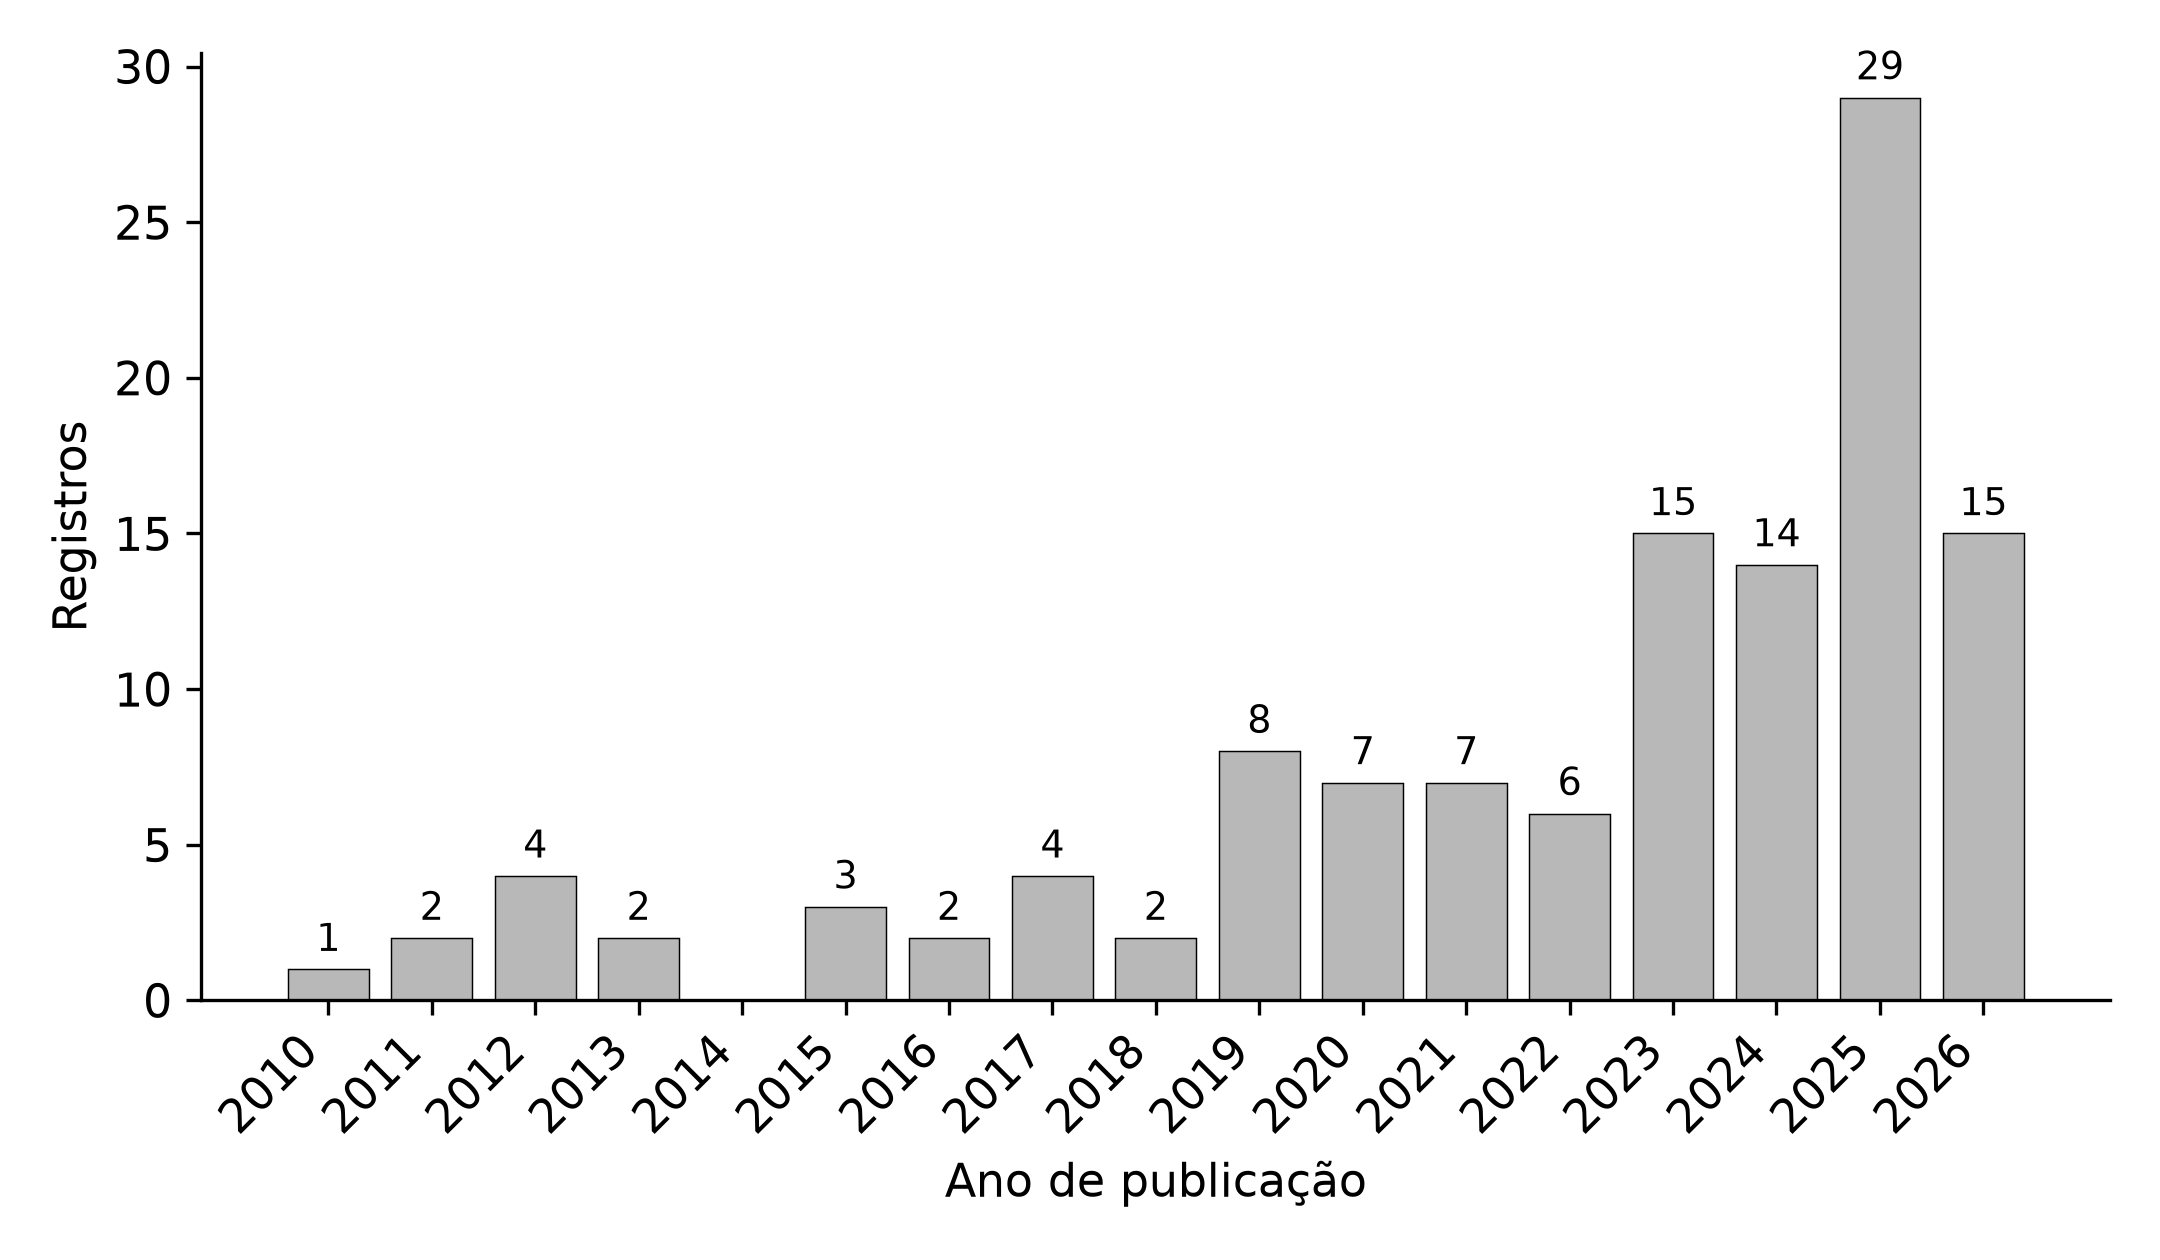
\includegraphics[width=0.9\linewidth]{figuras/figura09_distribuicao_temporal_nucleo_ampliado_121.png}
\captiongrafico{Distribuição temporal do núcleo temático vigente}
\label{fig:temporal}
\end{figure}

Os tipos documentais foram harmonizados, reunindo \textit{Journal}, \textit{JOUR} e \textit{journal-article} na categoria artigo de periódico; \textit{Conference Proceeding} e \textit{CPAPER} em trabalhos em evento; \textit{Book Series} e \textit{Book} em livro ou série de livro. A Tabela~\ref{tab:basetipo} apresenta proveniência e tipologia separadamente, indicando predomínio de artigos de periódico e forte presença da Scopus; a sobreposição entre bases registra caminhos de recuperação do mesmo estudo, enquanto a avaliação da evidência depende do conteúdo de cada registro.

\begin{table}[htbp]
\centering
\caption{Distribuição do núcleo temático vigente por base de origem e tipo documental}
\label{tab:basetipo}
\footnotesize
\begin{tabularx}{\textwidth}{>{\RaggedRight\arraybackslash}p{3.7cm} >{\raggedleft\arraybackslash}p{1.8cm} >{\raggedleft\arraybackslash}p{1.8cm} Y}
\toprule
Categoria & Registros & \% dos 121 & Observação \\
\midrule
\multicolumn{4}{l}{\textbf{A. Registros do núcleo com origem na base, respostas múltiplas}} \\
Scopus & 113 & 93,4 & Base bibliográfica principal. \\
Web of Science & 51 & 42,1 & Base bibliográfica independente. \\
Crossref & 6 & 5,0 & Fonte complementar de metadados. \\
\addlinespace
\multicolumn{4}{l}{\textbf{B. Tipo documental harmonizado, categorias exclusivas}} \\
Artigo de periódico & 90 & 74,4 & \textit{Journal}, \textit{JOUR} e \textit{journal-article}. \\
Trabalho em evento & 20 & 16,5 & \textit{Conference Proceeding} e \textit{CPAPER}. \\
Livro ou série de livro & 11 & 9,1 & \textit{Book Series} e \textit{Book}. \\
\bottomrule
\end{tabularx}
\fonteautor
\end{table}

A camada bibliométrica, com função analítica distinta da síntese temática (cf. Método), utilizou os 372 registros com aderência simultânea ao objeto predial, à manutenção ou gestão, à sustentabilidade e à presença de método, dados ou resultados; 329 (88,4\%) continham palavras-chave, 327 (87,9\%) DOI e 91 (24,5\%) autores. As palavras-chave foram normalizadas quanto a caixa, acentuação, singular e variantes ortográficas, reunindo, por exemplo, \textit{building information modeling}, \textit{building information modelling} e BIM; a rede considera a coocorrência no mesmo registro, normalizada pelo cosseno das frequências marginais, e a evolução compara 157 registros de 2010--2020 com 215 de 2021--2026.

O Gráfico~\ref{fig:fontes372} sintetiza 208 fontes, das quais o núcleo aproximado de Bradford reuniu 13, responsáveis por cerca de um terço dos registros, entre elas \textit{Energy and Buildings} (18), \textit{Journal of Building Engineering} (15), \textit{Facilities} (14), \textit{Lecture Notes in Civil Engineering} (11), \textit{IOP Conference Series: Earth and Environmental Science} (10) e \textit{Sustainability} (10), confirmando a interdisciplinaridade entre energia, engenharia de edificações, gestão de facilidades e sustentabilidade.

\begin{figure}[htbp]
\centering
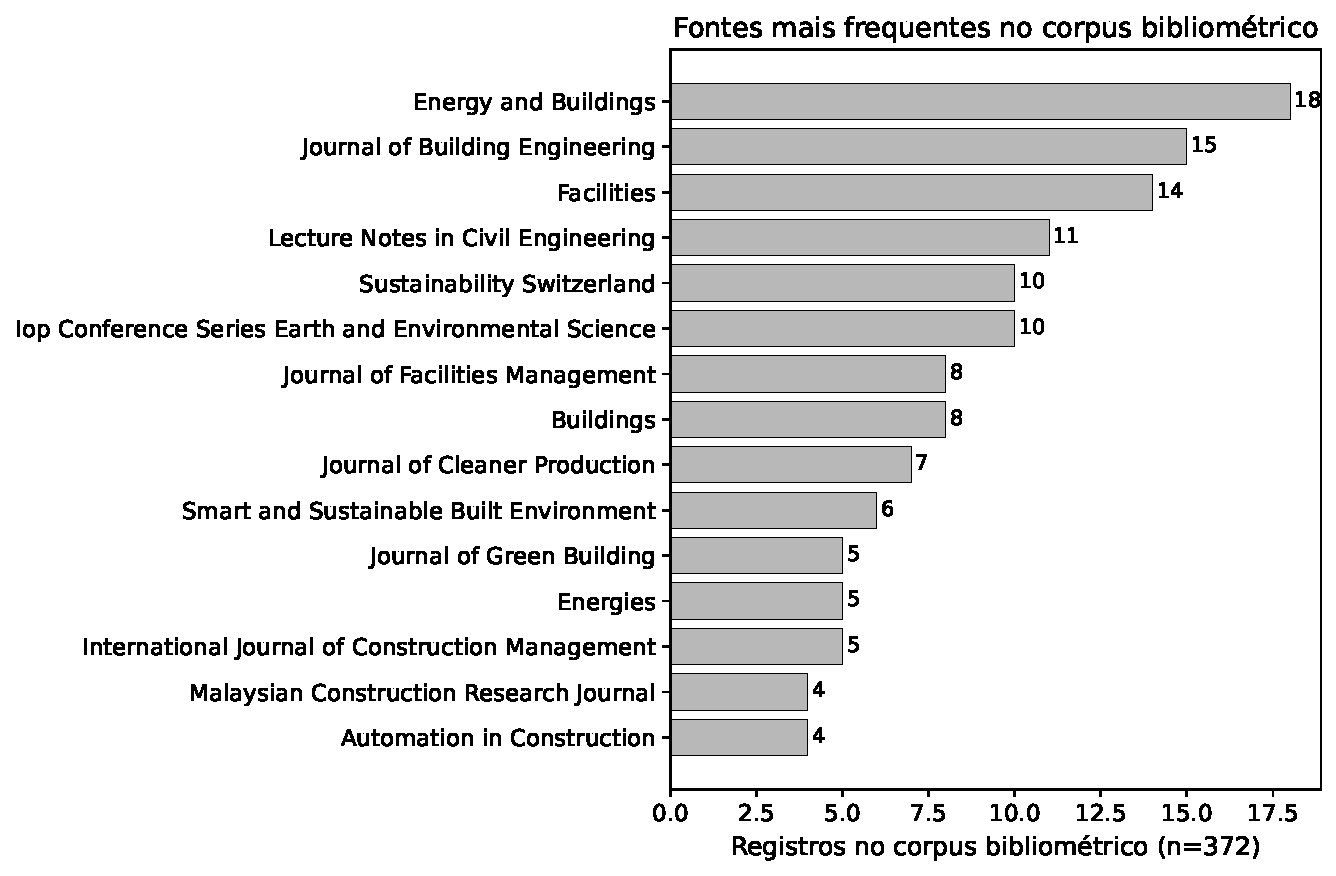
\includegraphics[width=0.98\linewidth]{figuras/figura_fontes_relevantes_372.pdf}
\captiongrafico{Fontes mais frequentes no corpus bibliométrico ampliado}
\label{fig:fontes372}
\end{figure}

O mapa temático (Gráfico~\ref{fig:mapatematico372}) revelou dois eixos centrais, formados por BIM, desempenho da edificação e \textit{digital twins}, com centralidade e densidade acima das medianas, e gestão de facilidades, edifícios inteligentes e manutenção preditiva, com elevada centralidade e menor densidade interna. Edificações verdes, avaliação do ciclo de vida e desenvolvimento sustentável formaram grupos mais especializados, enquanto energia, emissões e operação predial permaneceram semanticamente heterogêneas.

\begin{figure}[htbp]
\centering
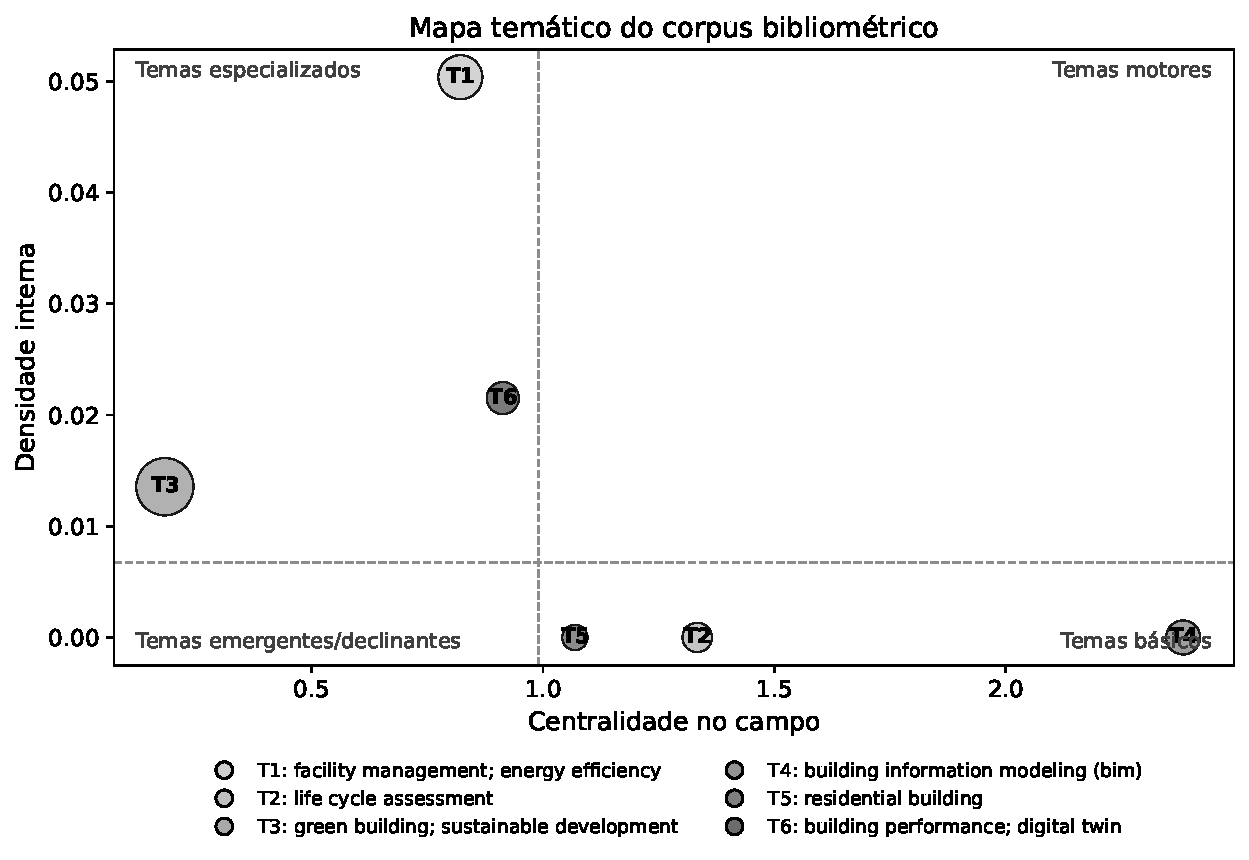
\includegraphics[width=0.98\linewidth]{figuras/figura_mapa_tematico_372.pdf}
\captiongrafico{Mapa temático por centralidade e densidade das palavras-chave}
\label{fig:mapatematico372}
\end{figure}

A rede normalizada (Gráfico~\ref{fig:redecor372}) reforça BIM e gestão de facilidades como conectores centrais, associados a \textit{digital twins}, manutenção preditiva, operação, desempenho, gestão de ativos e internet das coisas; em outro agrupamento, avaliação do ciclo de vida aproxima-se de edificações residenciais e desenvolvimento sustentável.

\begin{figure}[htbp]
\centering
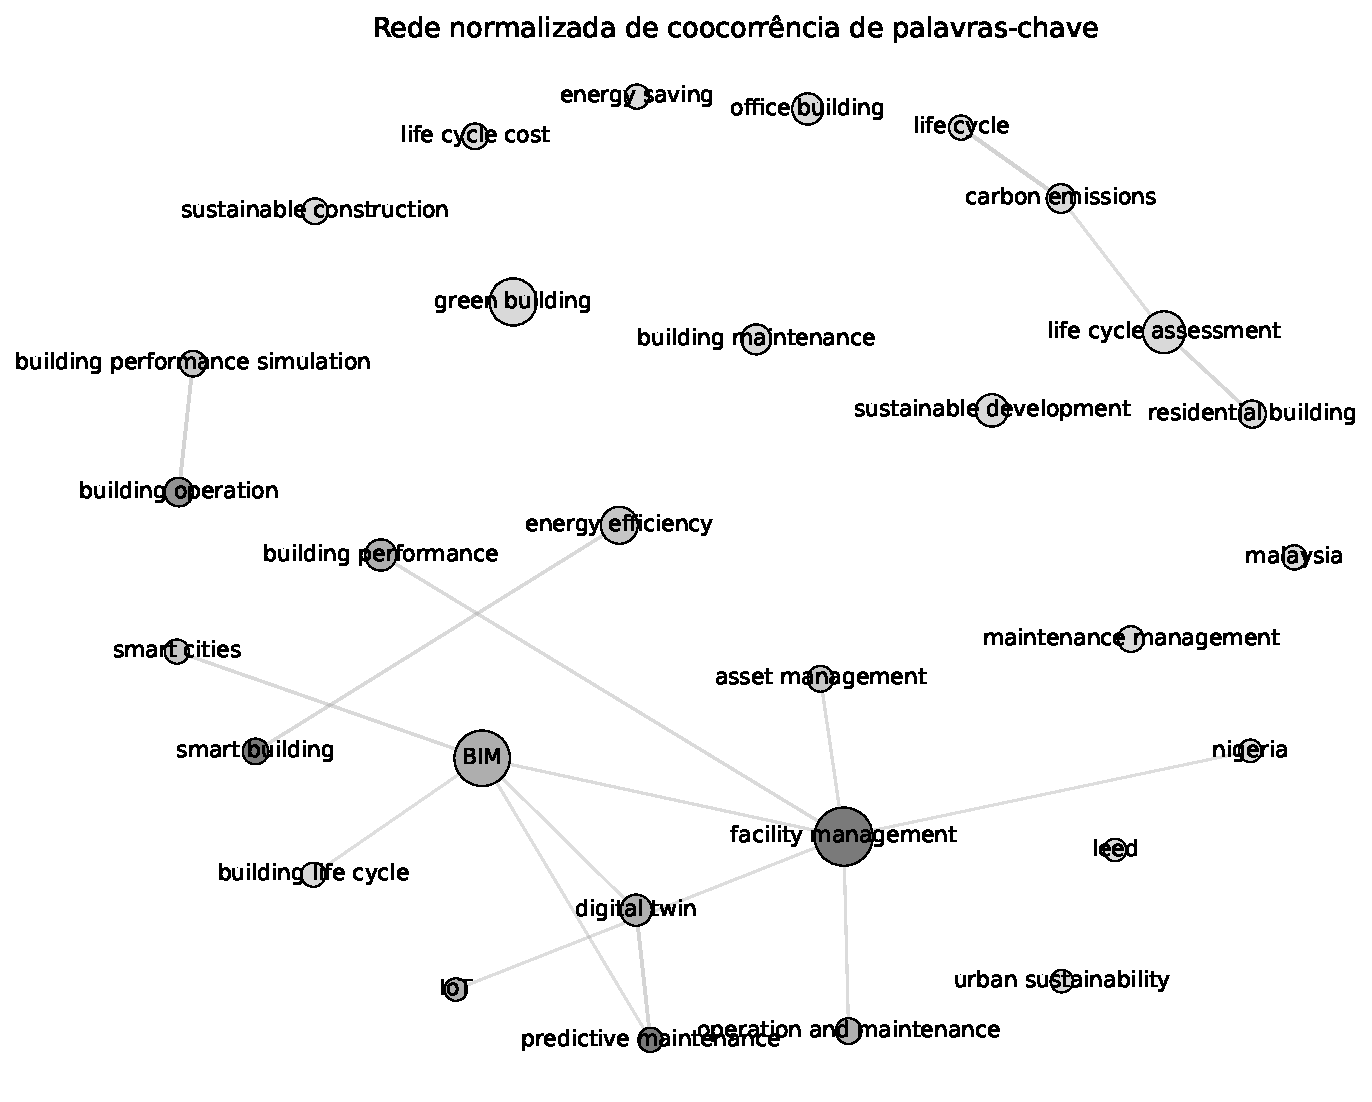
\includegraphics[width=0.98\linewidth]{figuras/figura_rede_coocorrencia_372.pdf}
\captiongrafico{Rede normalizada de coocorrência de palavras-chave}
\label{fig:redecor372}
\end{figure}

A comparação temporal (Gráfico~\ref{fig:evolucaotematica372}) mostrou aumento de 7,3 pontos percentuais para BIM, 4,7 para \textit{digital twins}, 2,7 para emissões de carbono e 1,9 para avaliação do ciclo de vida, enquanto edificação verde, eficiência energética, manutenção predial e desempenho da edificação perderam participação relativa. Esse movimento descreve uma associação documental de transição lexical, compatível com a incorporação de temas tradicionais a vocabulários tecnológicos e de ciclo de vida mais específicos, sem implicar relação causal entre os termos.

\begin{figure}[htbp]
\centering
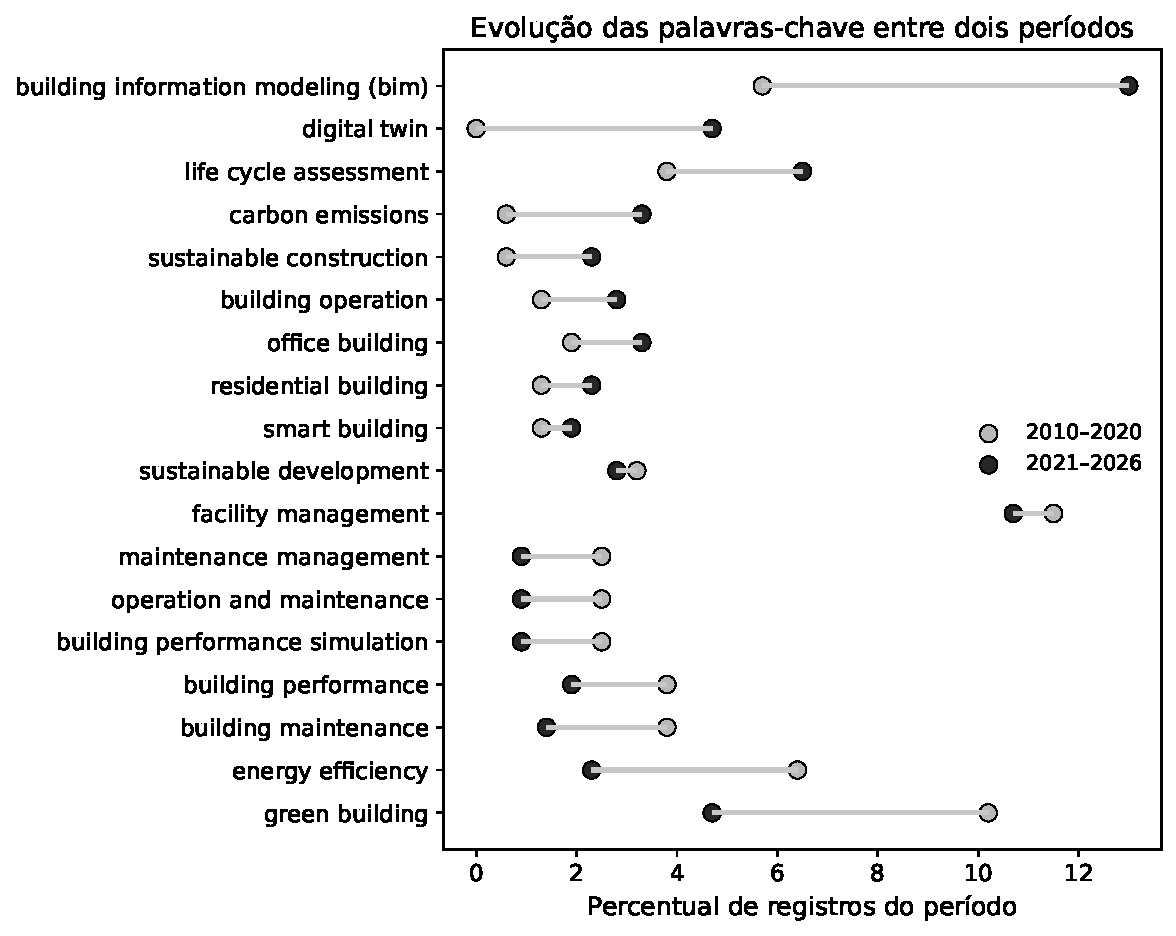
\includegraphics[width=0.98\linewidth]{figuras/figura_evolucao_tematica_372.pdf}
\captiongrafico{Evolução das palavras-chave entre 2010--2020 e 2021--2026}
\label{fig:evolucaotematica372}
\end{figure}

Em conjunto, a bibliometria indica transição de eficiência, desempenho e edificações verdes para BIM, \textit{digital twins}, carbono, ciclo de vida e manutenção preditiva, embora o crescimento informacional não implique, por si, integração decisória equivalente. As subseções seguintes verificam como essa transição se converte em dimensões, critérios, métodos e regras aplicáveis à priorização pública universitária.

\subsection{Dimensões e critérios para priorização sustentável}
\label{sec:criterios}

Foram identificadas seis dimensões com respostas múltiplas, na ordem técnica-operacional (116 registros), institucional (97), ambiental (92), ciclo de vida (65), econômica (63) e social (59). O predomínio das duas primeiras reflete a amplitude do manual de codificação e descreve a composição documental do núcleo, convergindo com a gestão sustentável de facilidades, que articula impactos ambientais, sociais e econômicos nos níveis estratégico, tático e operacional \parencite{nielsen_sustentabilidadefm_2016,okoro_sustainablefm_2023}, e com avaliações educacionais que integram desempenho, energia, conforto e usuários \parencite{alfalah_frameworkeducacional_2022}.

\begin{figure}[htbp]
\centering
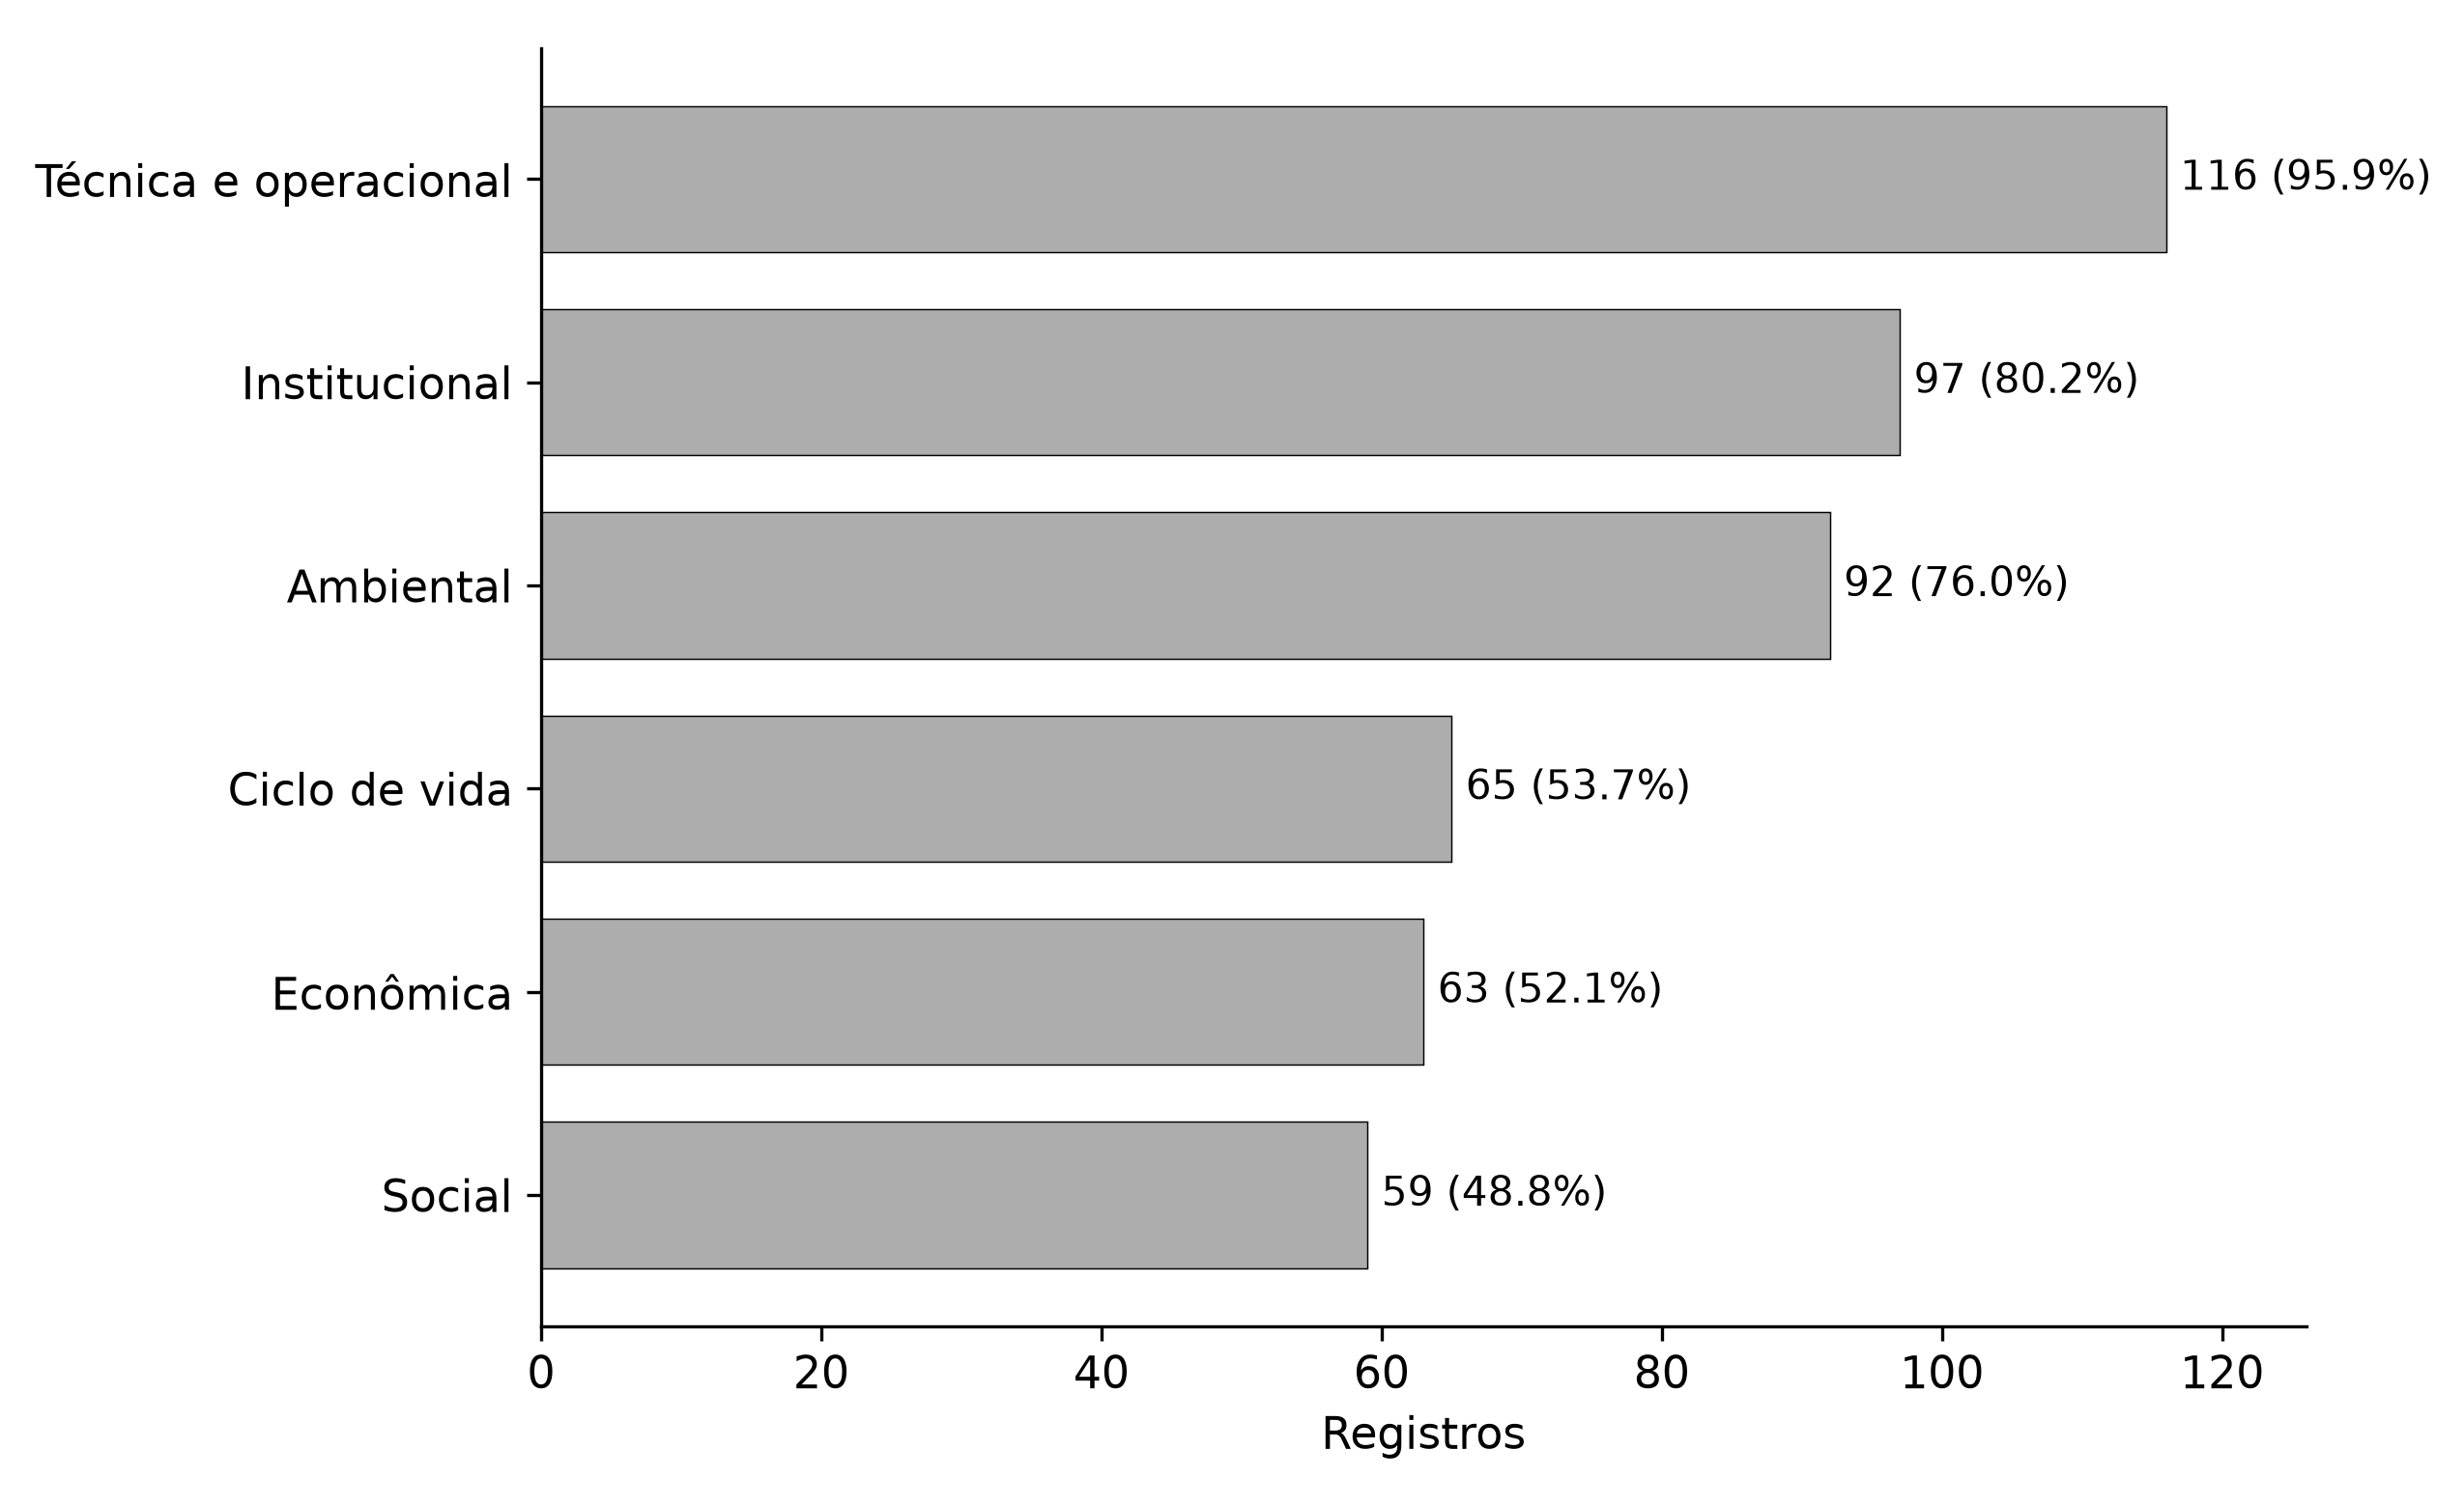
\includegraphics[width=0.90\linewidth]{figuras/figura12_dimensoes_sustentabilidade_nucleo_ampliado_121.png}
\captiongrafico{Dimensões de sustentabilidade identificadas no núcleo temático vigente}
\label{fig:dimensoes}
\end{figure}

Os ODS apareceram explicitamente em um registro, que combinou sustentabilidade, AHP, TOPSIS e otimização na alocação de prestadores de manutenção pública \parencite{masmoudi_ahptopsis_2026}; o vocabulário ESG esteve ausente dos campos auditados, embora componentes ambientais, sociais e institucionais fossem frequentes, padrão compatível com sua incorporação ainda emergente à gestão de facilidades \parencite{ramantswana_esgfm_2026}.

Quanto aos critérios de priorização, desempenho operacional apareceu em 99 registros, informação e dados em 82, custo em 63 e energia e vida útil em 44 cada, com os demais critérios técnicos, sociais e ambientais listados na Tabela~\ref{tab:criteriospriorizacao}.

\begin{table}[htbp]
\centering
\caption{Critérios de priorização identificados no núcleo temático vigente}
\label{tab:criteriospriorizacao}
\small
\begin{tabularx}{\textwidth}{Y >{\raggedleft\arraybackslash}p{2.1cm} >{\raggedleft\arraybackslash}p{2.1cm}}
\toprule
Critério & Registros & \% dos 121 \\
\midrule
Desempenho operacional & 99 & 81,8 \\
Informação e dados & 82 & 67,8 \\
Custo & 63 & 52,1 \\
Energia & 44 & 36,4 \\
Vida útil & 44 & 36,4 \\
Condição física & 34 & 28,1 \\
Risco & 33 & 27,3 \\
Manutenibilidade & 25 & 20,7 \\
Conforto & 22 & 18,2 \\
Segurança & 18 & 14,9 \\
Emissões de carbono & 15 & 12,4 \\
Resíduos & 13 & 10,7 \\
Satisfação do usuário & 9 & 7,4 \\
Água & 6 & 5,0 \\
Qualidade de serviço & 6 & 5,0 \\
\bottomrule
\end{tabularx}
\fonteautor
\end{table}

Na gestão pública universitária, o desempenho sustenta indicadores relacionados à continuidade e às falhas, a informação oferece as condições necessárias à rastreabilidade e o custo permite distinguir correções emergenciais, manutenção planejada e renovação, combinação reforçada por registros de pagamento e planejamento conjunto de manutenção, renovação e energia \parencite{kim_estimativacustoseducacional_2018,nageli_ciclovida_2019}. As leituras integrais qualificam relações entre critérios. Operação e manutenção podem superar 80\% do custo total do ciclo de vida, e seus custos anuais podem representar de 50\% a 70\% dos custos operacionais, bases de cálculo que devem permanecer distintas \parencite{aliu_barreirasdt_2025}; decisões de concepção podem evitar até 50\% das dificuldades de manutenção, conectando manutenibilidade a desempenho, custo e risco \parencite{othman_manutenibilidadeesi_2023,chew_manutenibilidadeverde_2016,conejos_verticalgreenery_2019}.

\subsection{Digitalização, IA e métodos de apoio à decisão}
\label{sec:metodos}

Sobre os métodos de apoio à decisão, a categoria ampla \texttt{framework} reuniu 101 registros. BIM apareceu em 28 e a categoria \texttt{decision\_support}, definida no manual como presença de mecanismo explícito de apoio à decisão, em 29; seguiram-se aprendizado de máquina em 26, otimização em 19, pontuação em 17 e custo do ciclo de vida em 16. Entre os métodos nomeados, AHP ocorreu em cinco registros, TOPSIS em quatro, MCDM e Delphi em três cada, ANP em dois, e \textit{Bayesian Best-Worst Method}, \textit{balanced scorecard} e raciocínio baseado em casos em um cada. Essa predominância de estruturas genéricas sobre métodos multicritério nomeados marca a transição do campo, cujo avanço informacional é mais rápido que a integração decisória.

\begin{figure}[htbp]
\centering
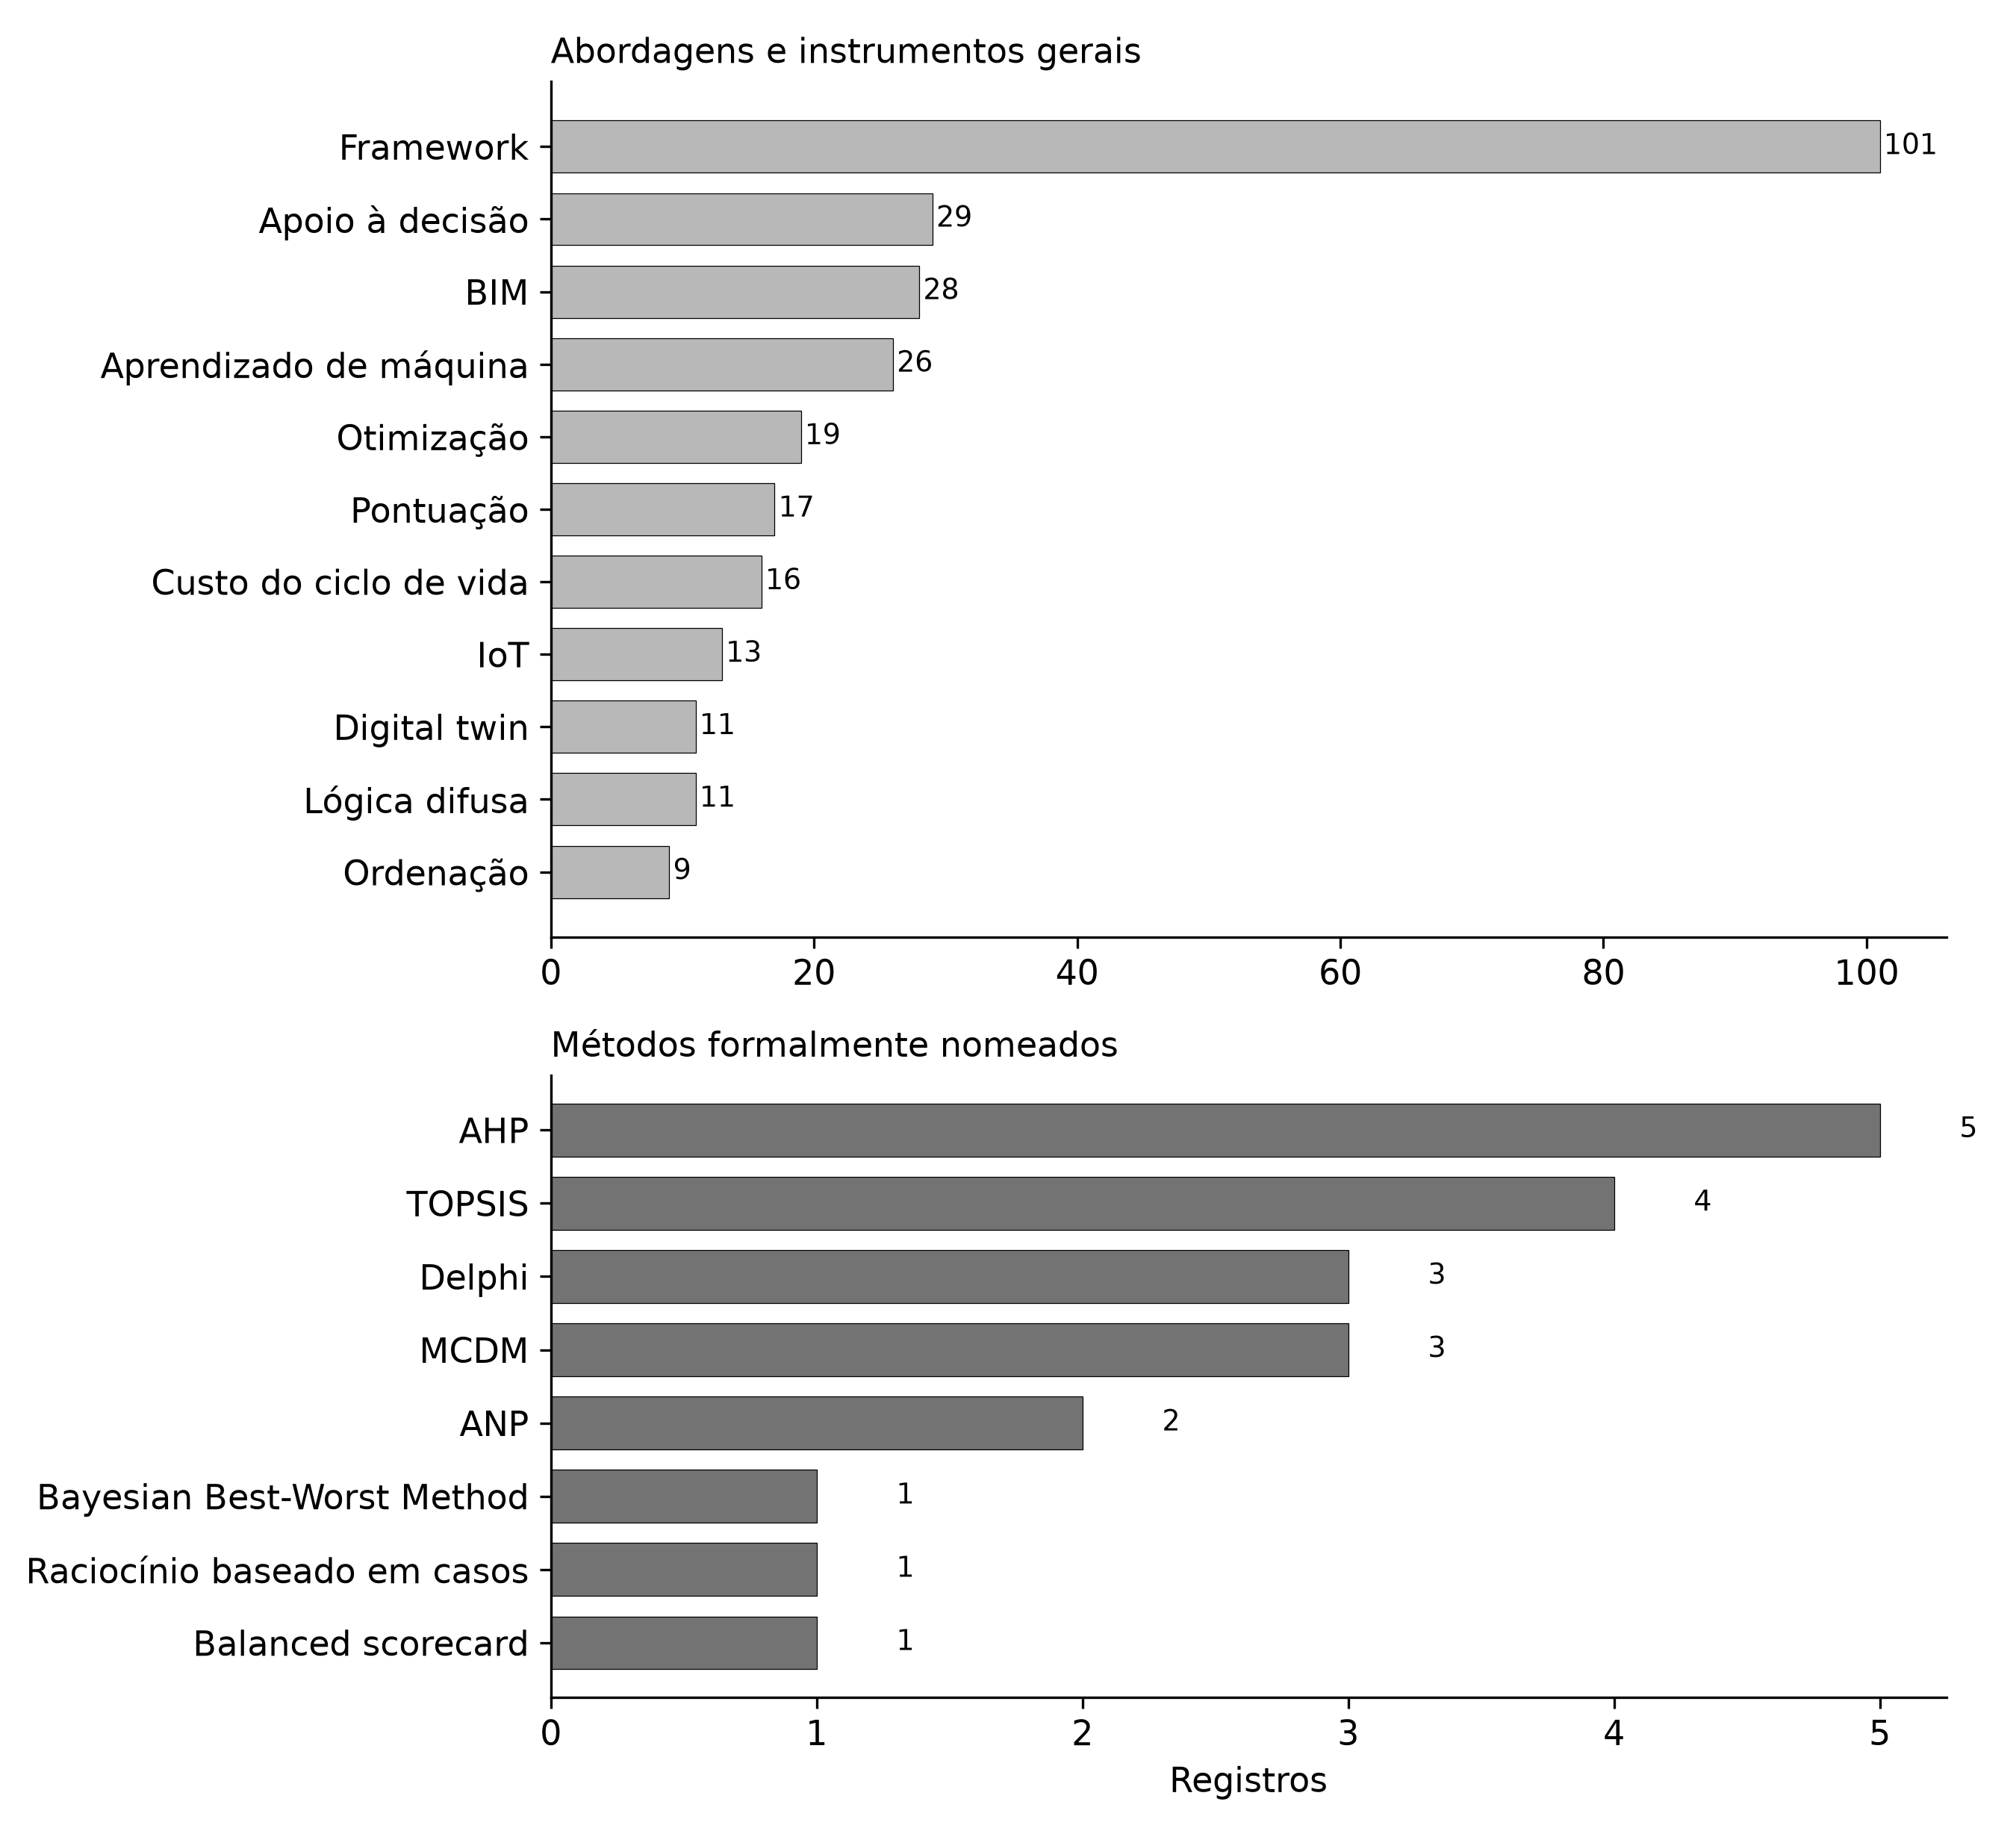
\includegraphics[width=0.95\linewidth]{figuras/figura11_metodos_mcdm_mais_frequentes_nucleo_ampliado_121.png}
\captiongrafico{Abordagens e métodos de apoio à decisão identificados no núcleo temático vigente}
\label{fig:metodos}
\end{figure}

\textit{Digital twin} foi identificado em 11 registros (9,1\%), e a busca de sensibilidade elevou o aprendizado de máquina de nove para 26 registros (21,5\%), resultado diretamente associado ao enriquecimento temático da rodada complementar. Para a especificação proposta, a arquitetura informacional pode começar com planilhas, cadastros, inspeções e ordens de serviço e evoluir para plataformas digitais e módulos preditivos conforme a qualidade dos dados. As aplicações multicritério identificadas desempenham funções distintas, como o ANP difuso na avaliação de edifícios educacionais \parencite{alfalah_frameworkeducacional_2022}, Delphi modificado na gestão de \textit{campus} \parencite{naji_campusdelphi_2023} e a combinação de AHP, TOPSIS e otimização na alocação de prestadores públicos \parencite{masmoudi_ahptopsis_2026}.

A leitura integral do lote da RQ6 separa produção de variáveis operacionais e governança decisória. Modelos de aprendizado de máquina estimaram demanda de ventilação, com economia de até 7,5\% sobre o controle tradicional \parencite{motuziene_ventilacaoia_2025}, vida útil de componentes por regressão em grafos, com $R^2=0{,}83$ \parencite{wu_gnnvidautil_2025}, e consumo de eletricidade, gás e água com conjuntos separados de treinamento, validação e teste \parencite{suh_demandaenergiaagua_2012}, além de diagnóstico, classificação de danos e apoio operacional. Duas revisões qualificam esse alcance. A síntese de IoT e IA identificou concentração no Norte Global e desafios de interoperabilidade, privacidade, governança e ciclo de vida \parencite{das_iotai_2025}, e entre 76 estudos sobre ambientes internos conectados, 41 integraram energia, conforto e sustentabilidade e 35 apenas parte delas \parencite{alici_iotambientes_2026}. A matriz comparativa dos 17 registros, no material suplementar, classifica dez estudos em previsão ou previsão com otimização, dois em diagnóstico e classificação de danos e cinco em síntese ou integração tecnológica, e apenas três aproximam a saída de uma ação operacional. A integração com preferências institucionais, ponderação e vetos permanece etapa decisória adicional.

As leituras do núcleo original ampliam essa distinção. A revisão de 123 estudos encontrou \textit{digital twins} em estágios parciais de controle, otimização e retroalimentação \parencite{deng_bimdigitaltwins_2021}, e outros trabalhos desenvolveram ontologia de ativos, BIM 7D e comparação de estratégias por simulação \parencite{gispert_ontologiaativos_2025,goretti_bimoem_2023,ferreira_manutencaoceramica_2020}. No plano decisório, aparecem Lean Six Sigma, avaliação sintética fuzzy e raciocínio baseado em casos com Fuzzy-AHP \parencite{aldairi_lean6sbm_2017,yoon_fuzzyfm_2018,park_cbrfuzzyahp_2019}, casos que distinguem menção conceitual, aplicação formal e validação empírica.

A presença de \texttt{framework} em quase todo o núcleo, contrastada com a frequência menor de métodos multicritério nomeados, situa a lacuna central na cadeia entre evidência, variável mensurável, preferência institucional e decisão validada, padrão coerente com a fragmentação já discutida entre integração informacional e estruturação decisória \parencite{deng_bimdigitaltwins_2021,das_iotai_2025}. Estruturas conceituais, indicadores, normalização, ponderação, agregação, sensibilidade e validação ocupam etapas distintas, e a transferência das aplicações de ANP, Delphi, AHP e TOPSIS à gestão universitária depende do contexto e dos dados locais. Nessa leitura, a barreira à adoção de métodos multicritério em universidades públicas tende a ser menos a complexidade algorítmica do que a cultura de registro, atualização cadastral e prestação de contas das escolhas, sustentada pela importância atribuída a ordens de serviço, custos, vínculo com ativos e histórico de intervenções \parencite{martins_custosmanutencaoses_2024,morais_eficienciamanutencao_2023}.

\subsection{Especificidade das edificações públicas universitárias}
\label{sec:aplicabilidade}

A caracterização documental identificou 101 registros sobre edificação genérica e 59 sobre portfólio predial. Entre as tipologias específicas, apareceram 17 hospitais, 16 edifícios comerciais, 15 residenciais, 14 universidades, dez \textit{campus}, seis patrimônios históricos, cinco edifícios públicos, cinco escolas e um museu, categorias que admitem respostas múltiplas (Tabela~\ref{tab:contexto}).

\begin{table}[htbp]
\centering
\caption{Contextos de edificação identificados no núcleo temático vigente}
\label{tab:contexto}
\small
\begin{tabularx}{\textwidth}{Y >{\raggedleft\arraybackslash}p{2.1cm} >{\raggedleft\arraybackslash}p{2.1cm}}
\toprule
Contexto & Registros & \% dos 121 \\
\midrule
Edificação genérica & 101 & 83,5 \\
Portfólio predial & 59 & 48,8 \\
Hospital & 17 & 14,0 \\
Edifício comercial & 16 & 13,2 \\
Edifício residencial & 15 & 12,4 \\
Universidade & 14 & 11,6 \\
\textit{Campus} & 10 & 8,3 \\
Patrimônio histórico & 6 & 5,0 \\
Edifício público & 5 & 4,1 \\
Escola & 5 & 4,1 \\
Museu & 1 & 0,8 \\
Não identificado no resumo & 1 & 0,8 \\
\bottomrule
\end{tabularx}
\fonteautor
\end{table}

Em instituições de ensino, a gestão sustentável combina desempenho físico, usuários e capacidade administrativa. Estudos em universidades públicas registraram predomínio corretivo, cadastros fragmentados, baixa institucionalização de indicadores e fragilidades na manutenção preventiva \parencite{lateef_manutencaouniversidade_2010,barbosa_facilitiesinstituicaopublica_2020}, e outros trabalhos identificaram fatores críticos em universidades \parencite{awuzie_fmuniversidades_2017}, critérios ambientais, econômicos e sociais em edifícios educacionais \parencite{alfalah_frameworkeducacional_2022}, indicadores operacionais de \textit{campus} \parencite{naji_campusdelphi_2023} e previsão orçamentária apoiada em ordens de serviço \parencite{martins_custosmanutencaoses_2024,morais_eficienciamanutencao_2023}. No contexto das universidades federais brasileiras, esse conjunto reforça a prioridade de cadastros consistentes, regras de veto e histórico dos parâmetros para a prestação de contas.

A análise das lacunas mostrou que 76 registros (62,8\%) apresentaram limitação identificável no resumo, enquanto 45 (37,2\%) não a explicitaram nesse nível documental. Doze registros (9,9\%) foram classificados no subconjunto específico de lacunas para instituições públicas de ensino superior, reunindo problemas de transferência, cobertura ou validação relacionados a essas instituições. A participação reduzida de universidades, \textit{campus} e edifícios públicos restringe a transferência direta para portfólios heterogêneos submetidos a contingenciamento, continuidade acadêmica e múltiplos usuários; a busca de sensibilidade elevou o contexto universitário de 11 para 14 registros, mas os três promovidos vieram do mesmo \textit{campus} da \textit{National Taiwan University}, ampliando a evidência tecnológica, e não a diversidade institucional.

Contextos africanos acrescentam resiliência, governança, usuários e continuidade acadêmica à condição física \parencite{awuzie_fmuniversidades_2017,ndukuba_resilienciainstitucional_2025}, hipóteses de transferência para validação brasileira. Em texto completo, um instrumento estrangeiro exigiu adaptação para aplicação em hospital público \parencite{talib_hospitalfm_2013}, e outros três projetos identificaram perdas de informação entre construção e operação, recorrendo ao BIM, à entrega suave (\textit{Soft Landings}) e à comunicação \parencite{tan_fluxoinformacao_2018}. Essas evidências sustentam governança da informação e validação contextual da especificação proposta a seguir.

\subsection{Da evidência à especificação operacional}
\label{sec:matriz}

O Gráfico~\ref{fig:heatmap} apresenta as coocorrências documentais entre os dez critérios e os dez instrumentos de apoio à decisão mais frequentes. Desempenho operacional e \texttt{framework} aparecem juntos em 90 registros, informação e dados têm 75 coocorrências com \texttt{framework} e 28 com BIM, custo associa-se a \texttt{framework} em 57 registros, e vida útil e custo do ciclo de vida apresentam 16 coocorrências. Essas relações descrevem associações de codificação e orientam a análise das combinações recorrentes.

\begin{figure}[htbp]
\centering
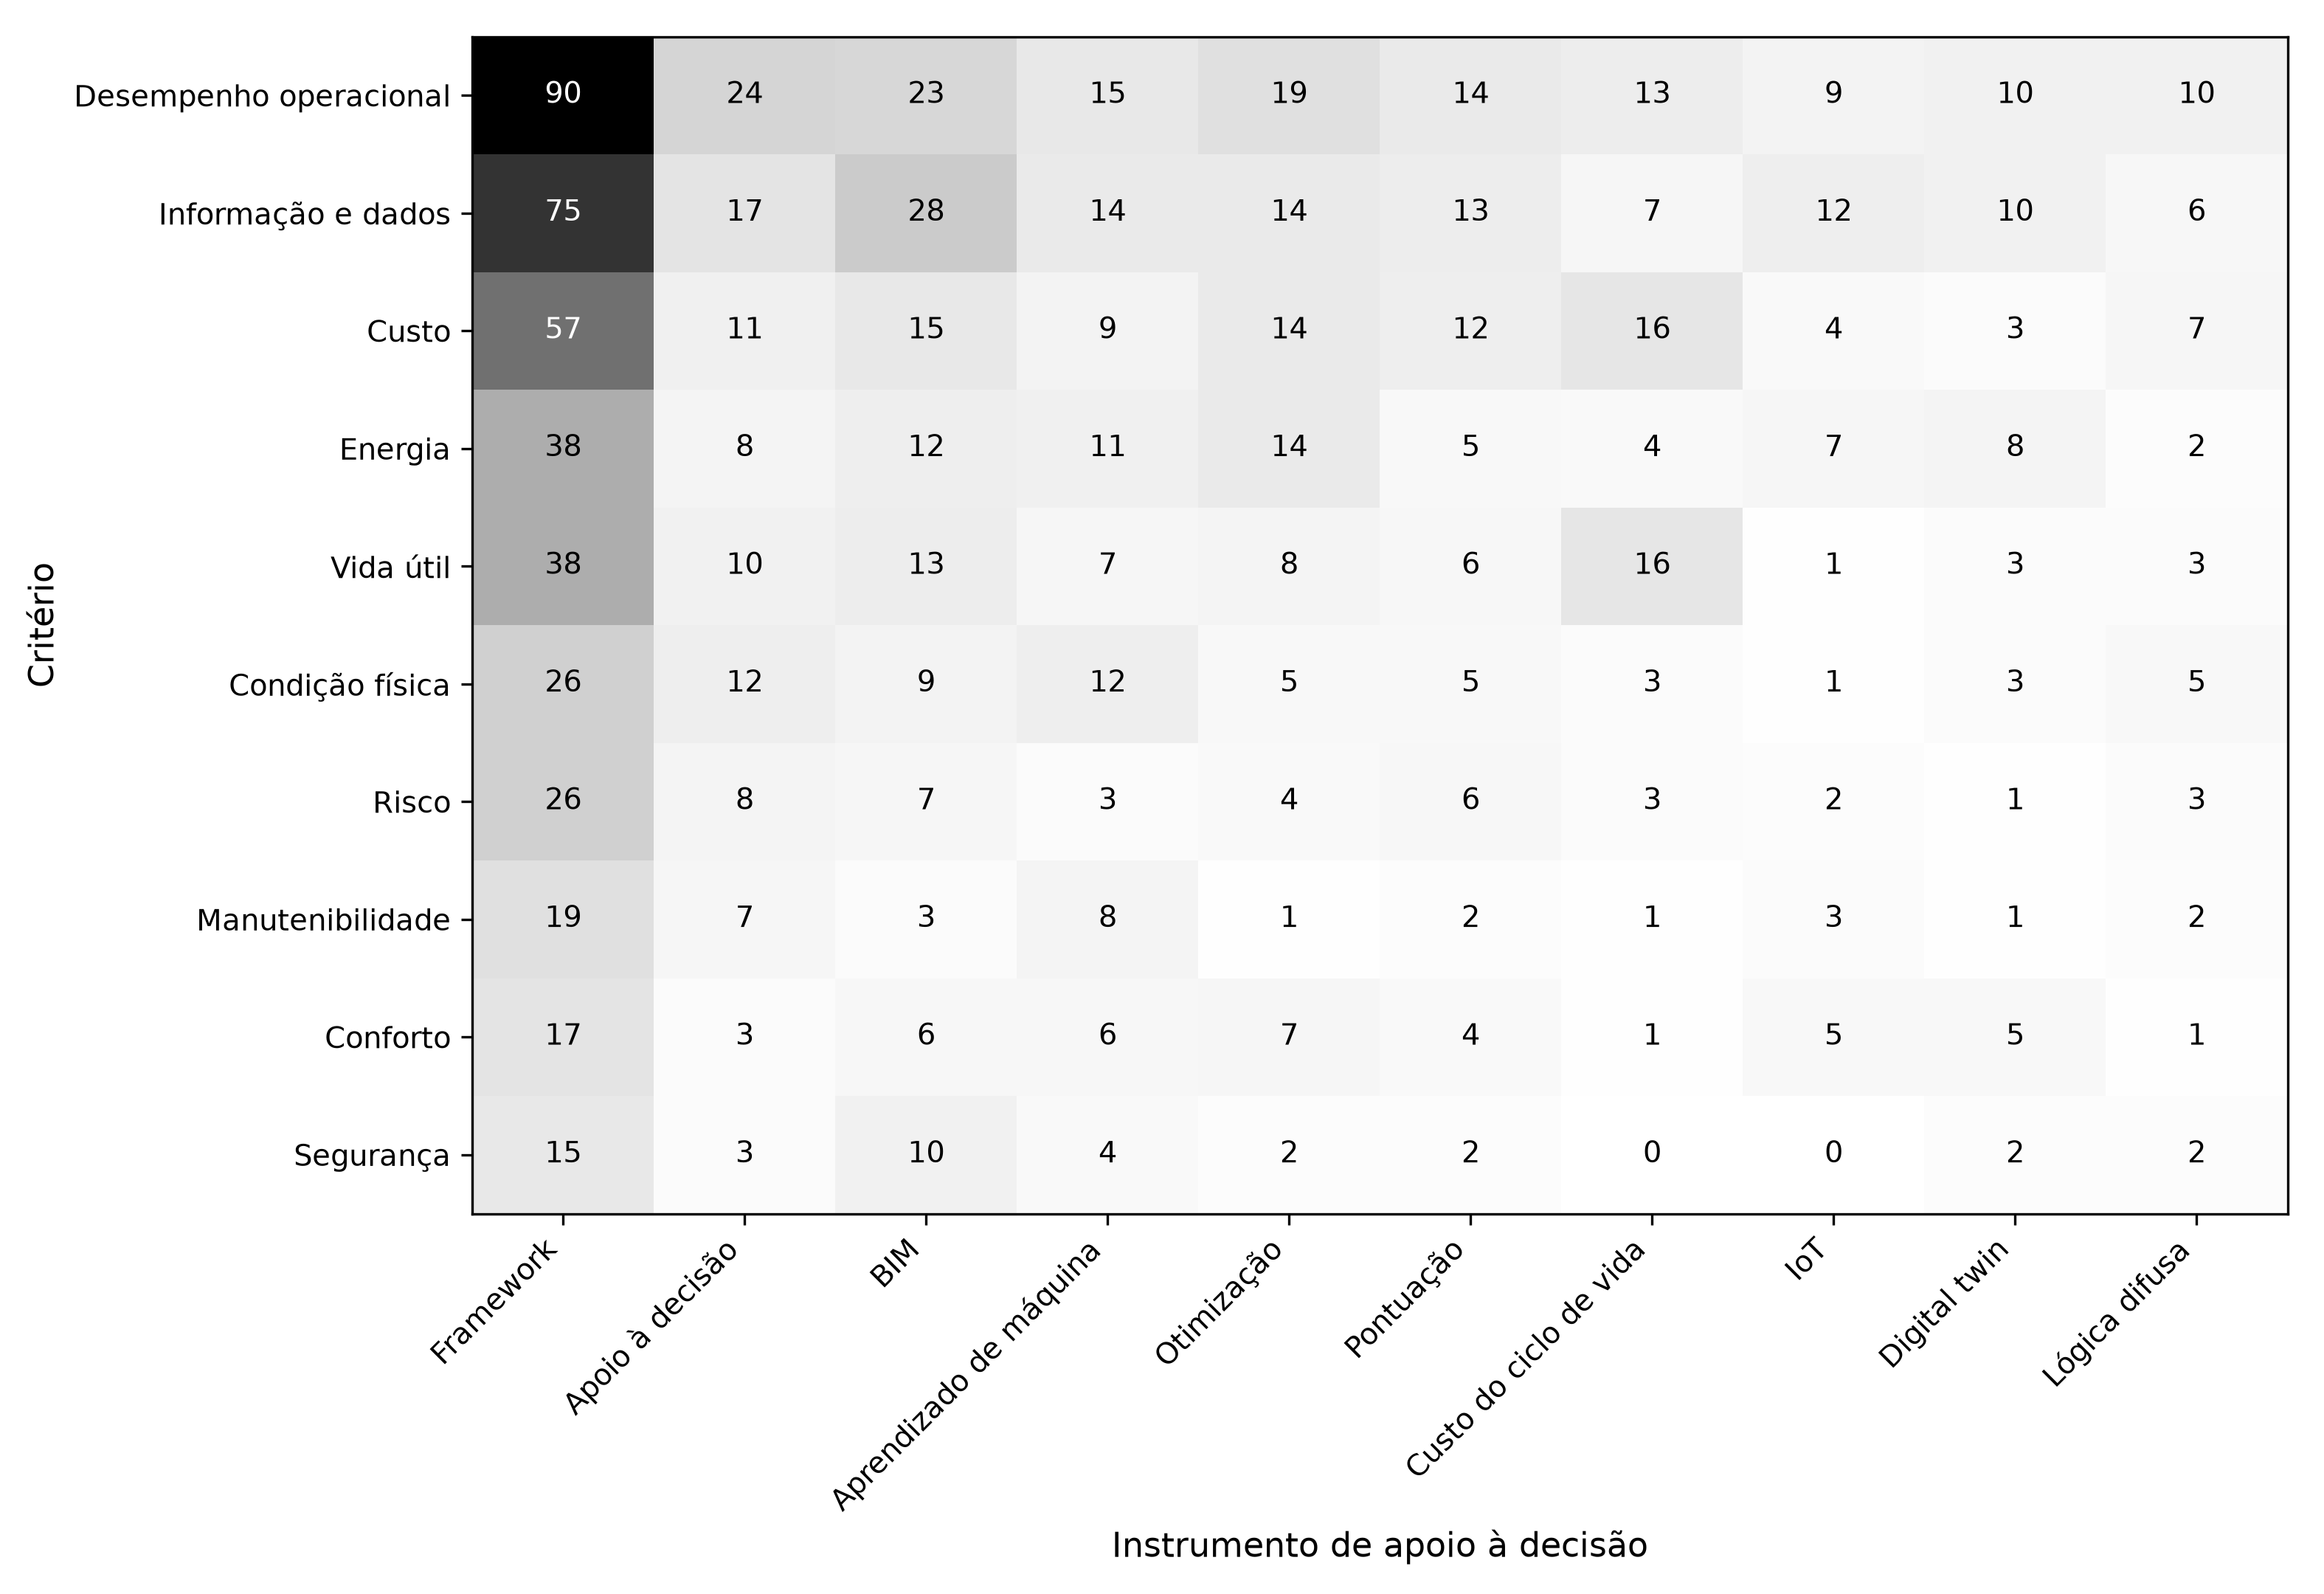
\includegraphics[width=0.98\linewidth]{figuras/figura13_heatmap_criterios_metodos_nucleo_ampliado_121.png}
\captiongrafico{Coocorrência entre critérios de priorização e instrumentos de apoio à decisão}
\label{fig:heatmap}
\end{figure}

O Gráfico~\ref{fig:matrizanalitica} reorganiza essas relações em cinco dimensões. A técnica-operacional apresenta 100 coocorrências com \texttt{framework}, 28 com \texttt{decision\_support} e 28 com BIM; em relação ao \texttt{framework}, a institucional apresenta 88 coocorrências, a ambiental 81, a econômica 56 e a social 54; identificada em 65 registros, a dimensão ciclo de vida atua transversalmente entre desempenho, custos e impactos no tempo.

\begin{figure}[htbp]
\centering
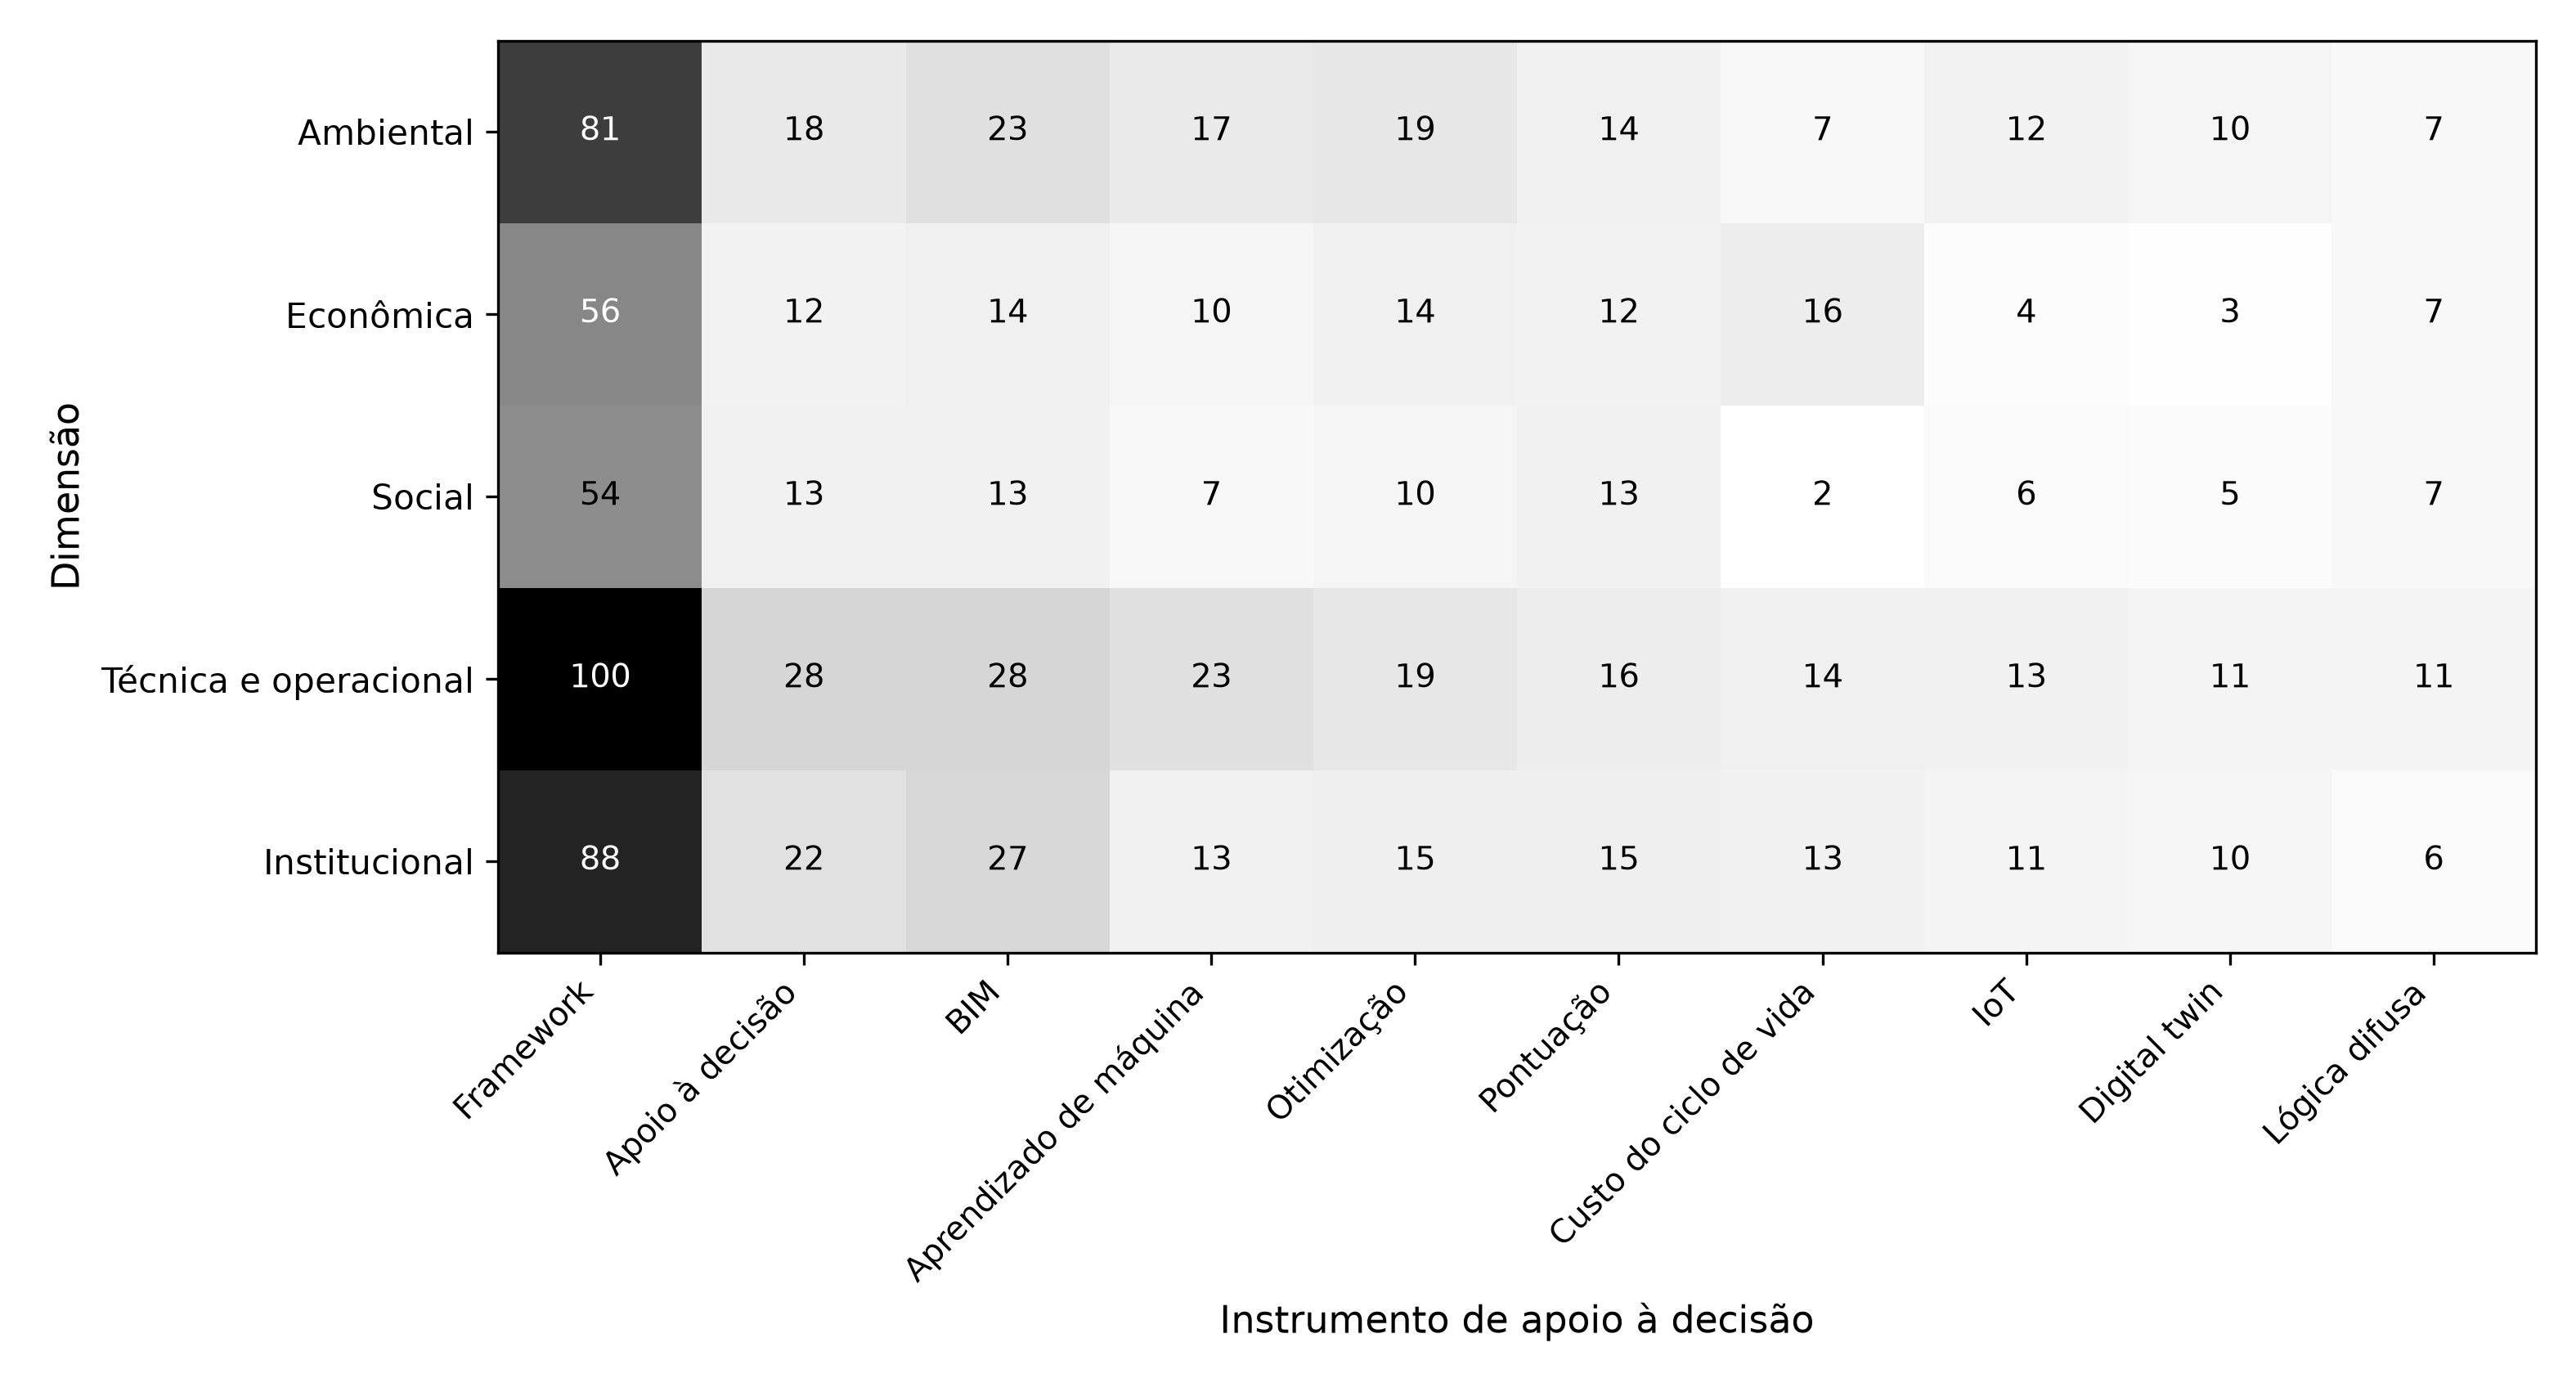
\includegraphics[width=0.98\linewidth]{figuras/figura14_matriz_analitica_dimensao_metodo_nucleo_ampliado_121.png}
\captiongrafico{Matriz de coocorrência entre dimensões de sustentabilidade e instrumentos de apoio à decisão}
\label{fig:matrizanalitica}
\end{figure}

A matriz que segue é uma síntese conceitual informada pela revisão, e não é um modelo validado nem um instrumento pronto para decisão; ela separa evidência extraída e especificação autoral. A dimensão ambiental reúne energia, emissões, água e resíduos, o custo constitui a dimensão econômica, segurança, conforto e satisfação integram a dimensão social, a técnica-operacional abrange desempenho, informação, vida útil, risco, condição, manutenibilidade e qualidade do serviço, e a institucional, presente em 97 registros, fundamenta os desdobramentos candidatos de conformidade, governança e capacidade de execução. As frequências sustentam a seleção inicial, enquanto pesos e importância normativa serão definidos na validação institucional. A Tabela~\ref{tab:protocolooperacional} liga critérios candidatos às evidências da revisão, e a Tabela~\ref{tab:especificacaoindicadores} apresenta, em plano separado, indicadores, fontes, periodicidades e direções propostos pelo autor para validação.

\begin{table}[htbp]
\centering
\caption{Rastreabilidade entre evidências e critérios candidatos}
\label{tab:protocolooperacional}
\scriptsize
\begin{tabularx}{\textwidth}{>{\RaggedRight\arraybackslash}p{2.4cm} >{\RaggedRight\arraybackslash}p{2.7cm} Y}
\toprule
Dimensão & Critério & Evidência da revisão \\
\midrule
Técnica-operacional & Desempenho e falha & Desempenho em 99 registros. A rede conecta gestão de facilidades a operação e manutenção. \\
Técnica-operacional & Informação e dados & Informação em 82 registros, BIM em 28 e \textit{digital twin} em 11. Perdas de informação foram observadas por \textcite{tan_fluxoinformacao_2018}. \\
Técnica-operacional & Condição e vida útil & Condição em 34 registros, vida útil em 44 e ciclo de vida em 65. A manutenibilidade é apoiada por \textcite{othman_manutenibilidadeesi_2023}. \\
Institucional & Conformidade & Dimensão institucional em 97 registros. \textcite{talib_hospitalfm_2013} aponta a necessidade de adaptação contextual. \\
Econômica & Custo & Custo em 63 registros. Previsão e ciclo de vida aparecem em \textcite{kim_estimativacustoseducacional_2018,nageli_ciclovida_2019}. \\
Ambiental & Energia & Dimensão ambiental em 92 registros e energia em 44. Ciclo de vida e carbono cresceram no período recente. \\
Social & Impacto nos usuários & Dimensão social em 59 registros, com conforto em 22, segurança em 18 e satisfação em nove. \\
\bottomrule
\end{tabularx}
\fonteautor
\end{table}

\begin{table}[htbp]
\centering
\caption{Proposição autoral de especificação operacional dos indicadores}
\label{tab:especificacaoindicadores}
\footnotesize
\begin{tabularx}{\textwidth}{>{\RaggedRight\arraybackslash}p{2.15cm} Y >{\RaggedRight\arraybackslash}p{2.3cm} >{\RaggedRight\arraybackslash}p{1.55cm} >{\RaggedRight\arraybackslash}p{1.7cm}}
\toprule
Critério & Indicador candidato & Fonte candidata & Apuração & Preferência \\
\midrule
Desempenho e falha & Ordens recorrentes por sistema, \% das ordens & Ordens de serviço & Mensal & Menor \\
Informação e dados & Ativos com cadastro e histórico completos, \% & Cadastro e ordens & Trimestral & Maior \\
Condição e vida útil & Índice de condição, escala institucional & Inspeção e cadastro & Semestral & Maior \\
Conformidade & Requisitos atendidos, \% & Laudos e auditorias & Anual & Maior \\
Custo & Custo estimado por área, R\$/m$^2$ & Orçamentos institucionais e base oficial aplicável & Semestral & Menor \\
Energia & Intensidade energética em base móvel de 12 meses, kWh/m$^2$ & Faturas ou medidores & Mensal & Menor \\
Impacto nos usuários & Reclamações por 100 usuários & Ouvidoria e chamados & Trimestral & Menor \\
\bottomrule
\end{tabularx}
\par\smallskip{\footnotesize Nota: indicadores, unidades, fontes, periodicidades e direções são proposições do autor para validação institucional. A revisão sustenta os critérios e a necessidade de rastreabilidade. Maior ou menor indica a direção desejável do indicador.\par}
\end{table}

A Figura~\ref{fig:fluxoprotocolo} resume o fluxo candidato, em que a unidade de comparação precede a coleta, e os critérios e indicadores são validados antes da elicitação dos pesos, com a divulgação da prioridade ocorrendo após a análise de sensibilidade e o registro das escolhas.

\begin{figure}[htbp]
\centering
\begin{tikzpicture}[
  node distance=7mm and 7mm,
  etapa/.style={draw, rounded corners, align=center, text width=3.6cm, minimum height=10mm, font=\scriptsize},
  veto/.style={draw, rounded corners, very thick, align=center, text width=11.7cm, minimum height=8mm, font=\scriptsize},
  seta/.style={-Latex, thick}
]
\node[etapa] (e1) {1. Definir unidade decisória};
\node[etapa, right=of e1] (e2) {2. Validar critérios e indicadores};
\node[etapa, right=of e2] (e3) {3. Verificar qualidade dos dados};
\node[etapa, below=of e3] (e4) {4. Parametrizar normalização, pesos e agregação};
\node[etapa, left=of e4] (e5) {5. Aplicar vetos e sensibilidade};
\node[etapa, left=of e5] (e6) {6. Registrar e publicar a prioridade};
\node[veto, below=of e5] (v) {Considera-se candidato a veto não compensatório qualquer risco estrutural, risco à vida, risco de incêndio ou descumprimento legal situado acima de limiar técnico ou normativo};
\draw[seta] (e1) -- (e2);
\draw[seta] (e2) -- (e3);
\draw[seta] (e3) -- (e4);
\draw[seta] (e4) -- (e5);
\draw[seta] (e5) -- (e6);
\draw[seta] (e5) -- (v);
\end{tikzpicture}
\caption{Fluxo candidato para validação e futura parametrização multicritério}
\label{fig:fluxoprotocolo}
\end{figure}

Na etapa 4, método, pesos e função de agregação serão definidos conforme o problema decisório, a participação institucional, a qualidade dos dados e o grau de compensação admissível. A análise de sensibilidade varia pesos, limiares e tratamento de ausências. Risco estrutural, risco à vida, incêndio e descumprimento legal formam vetos candidatos, com limiares estabelecidos por norma, laudo ou autoridade competente \parencite{abnt_nbr5674_2012,araujoneto_manutencaolegislacao_2015}; o ciclo de vida permanece transversal para evitar dupla contagem.

A especificação proposta liga, assim, os critérios sustentados pela revisão a indicadores candidatos e a um fluxo de validação, convertendo dimensões e critérios recorrentes em etapas verificáveis e respondendo à RQ0. A baixa presença lexical de ODS e ESG, diante da recorrência de energia, emissões, segurança, conforto e governança, indica aproximação substantiva ainda pouco expressa por esses rótulos \parencite{ramantswana_esgfm_2026}. As coocorrências descrevem associações documentais, e a avaliação institucional determinará importância, pesos, método e robustez segundo a força e a disponibilidade dos dados, completando a cadeia entre evidência científica, dimensão, critério, indicador observável, parametrização multicritério futura, veto não compensatório e decisão pública rastreável.

\section{Considerações finais}
\label{sec:consideracoes}

A pergunta central foi respondida pela integração de duas camadas parcialmente sobrepostas. O mapeamento bibliométrico identificou evolução temática de eficiência e desempenho para tecnologias digitais, carbono, ciclo de vida e manutenção preditiva; a síntese temática mostrou que as dimensões técnica-operacional, institucional e ambiental e os critérios de desempenho, informação, custo, vida útil, energia e risco formam o núcleo documental, com 109 dos 121 registros temáticos pertencendo também ao estrato bibliométrico de 372. Essa integração fundamentou a matriz de critérios e indicadores e o fluxo de validação para futura parametrização multicritério, respondendo à RQ0 ao ligar evidência, critérios e decisão pública rastreável.

Os resultados sugerem que a lacuna não está na escassez de dados, estruturas ou modelos, mas na cadeia que os conecta a uma decisão institucional validada. Estruturas genéricas, BIM e apoio à decisão foram mais frequentes que métodos multicritério nomeados, e a busca de sensibilidade, ao elevar o aprendizado de máquina de nove para 26 registros, revelou um lote de 17 estudos concentrado em previsão, diagnóstico e integração tecnológica, sem demonstrar uma cadeia decisória completa entre modelo treinado, validação externa, ponderação, vetos e decisão pública auditável. Universidades, \textit{campus} e edifícios públicos foram menos frequentes que edificações genéricas e portfólios, e doze registros apresentaram lacunas específicas para instituições públicas de ensino superior, reforçando a necessidade de validação contextual brasileira.

Diante dessa lacuna, a especificação operacional candidata acrescenta uma matriz rastreável que liga critérios sustentados pela revisão a indicadores, fontes, periodicidades e direções propostos pelo autor, além de um fluxo que ordena validação de conteúdo, normalização, ponderação, agregação e vetos candidatos. A revisão sustenta os critérios; os indicadores permanecem proposições autorais para validação, e a definição de pesos, agregação e limiares dos vetos de risco estrutural, risco à vida, risco de incêndio e descumprimento legal integra a etapa institucional seguinte, dependente de norma, laudo ou autoridade competente.

Essas dependências refletem também os limites do desenho adotado. A cobertura em Scopus, Web of Science e Crossref, entre 2010 e 2026 com o último ano parcial, priorizou metadados bibliográficos interoperáveis e deixou para estudos futuros pré-registro, rastreamento de citações e busca estruturada de literatura cinzenta; triagem e codificação foram conduzidas por um único avaliador, com decisões e regras preservadas para auditoria, e o enriquecimento deliberado da busca de sensibilidade para IA e aprendizado de máquina mede ganho de cobertura temática, não prevalência independente dessas técnicas. O núcleo de 121 registros foi sintetizado predominantemente por título, resumo, palavras-chave e campos estruturados, qualificado por 37 leituras integrais, das quais 19 acrescentaram evidências específicas. A unidade quantitativa é o registro consolidado, e publicações relacionadas podem compartilhar dados ou casos; a classificação do desenho permaneceu indeterminada em 23,1\% dos registros, e a revisão priorizou caracterização documental em vez de avaliação formal de risco de viés.

A continuidade do trabalho deverá começar pela validação de conteúdo, com a participação das áreas de manutenção, engenharia, sustentabilidade, planejamento e orçamento, além dos usuários, na revisão das dimensões, dos indicadores e dos vetos antes da elicitação dos pesos. Em seguida, ordens de serviço, inspeções, custos, consumo, riscos e reclamações deverão receber dicionário, periodicidade e responsáveis, para que o protótipo parametrize e teste o método de elicitação, a normalização, os pesos, a agregação, os limiares e a análise de sensibilidade, comparando estabilidade e utilidade decisória entre unidades e outros portfólios públicos.

Diante da escassez de recursos, esta especificação oferece um caminho possível para justificar cada investimento por critérios documentados e auditáveis, contribuindo para deslocar a priorização da manutenção de uma resposta improvisada para uma prática mais próxima da governança e do valor público, uma vez validada institucionalmente.

\subsection{Disponibilidade de dados}
\label{sec:disponibilidadedados}

Os dados brutos, intermediários e finais que sustentam esta revisão (protocolo de busca, matrizes de triagem e deduplicação, síntese temática e listas de referências em cada estágio) estão depositados em repositório aberto \parencite{oliveira_dadosuplementares_2026}.


\printbibliography[title={Referências}]

\end{document}
